% =====================================================================
%  CompLB3D User Guide
%  Build with:  pdflatex main && pdflatex main   (twice, for the TOC)
% =====================================================================
\documentclass[11pt,a4paper]{report}

\usepackage[T1]{fontenc}
\usepackage[utf8]{inputenc}
\usepackage{lmodern}
\usepackage{amsmath}
\usepackage{amssymb}
\usepackage{microtype}
\usepackage[margin=2.4cm,top=2.6cm,bottom=2.6cm]{geometry}
\usepackage{graphicx}
\usepackage{booktabs}
\usepackage{longtable}
\usepackage{array}
\usepackage{enumitem}
\usepackage{xcolor}
\usepackage{listings}
\usepackage{tcolorbox}
\usepackage{tikz}
\usepackage{fancyhdr}
\usepackage{titlesec}
\usepackage[hidelinks,bookmarksnumbered]{hyperref}
\usetikzlibrary{shapes.geometric,arrows.meta,positioning,fit,backgrounds,calc,decorations.pathreplacing}
\tcbuselibrary{skins,breakable}

% ---------------------------------------------------------------- colours
\definecolor{cbBlue}{HTML}{1F4E79}
\definecolor{cbTeal}{HTML}{2E7D74}
\definecolor{cbSand}{HTML}{F5F2EC}
\definecolor{cbRule}{HTML}{C8C2B6}
\definecolor{cbRed}{HTML}{9C3B2E}
\definecolor{cbGrey}{HTML}{5A5A5A}
\definecolor{cbCode}{HTML}{F7F7F4}

% ---------------------------------------------------------------- headings
\titleformat{\chapter}[display]
  {\normalfont\Large\bfseries\color{cbBlue}}
  {\filright\normalsize\color{cbGrey}\MakeUppercase{\chaptertitlename}\ \thechapter}
  {6pt}{\Huge\color{cbBlue}}
\titlespacing*{\chapter}{0pt}{0pt}{28pt}
\titleformat{\section}{\normalfont\large\bfseries\color{cbBlue}}{\thesection}{0.7em}{}
\titleformat{\subsection}{\normalfont\normalsize\bfseries\color{cbTeal}}{\thesubsection}{0.7em}{}

\pagestyle{fancy}
\fancyhf{}
\renewcommand{\headrulewidth}{0.4pt}
\fancyhead[L]{\small\color{cbGrey}\leftmark}
\fancyhead[R]{\small\color{cbGrey}CompLB3D User Guide}
\fancyfoot[C]{\small\thepage}
\fancypagestyle{plain}{\fancyhf{}\fancyfoot[C]{\small\thepage}\renewcommand{\headrulewidth}{0pt}}

% ---------------------------------------------------------------- listings
\lstdefinestyle{cbstyle}{
  basicstyle=\ttfamily\footnotesize,
  backgroundcolor=\color{cbCode},
  frame=leftline, framerule=1.6pt, rulecolor=\color{cbRule},
  framexleftmargin=5pt, xleftmargin=8pt,
  breaklines=true, breakatwhitespace=false,
  showstringspaces=false,
  keywordstyle=\color{cbBlue}\bfseries,
  commentstyle=\color{cbTeal}\itshape,
  stringstyle=\color{cbRed},
  columns=fullflexible, keepspaces=true,
  aboveskip=8pt, belowskip=8pt,
}
\lstset{style=cbstyle}
\lstdefinelanguage{xmlish}{
  morestring=[b]",
  morecomment=[s]{<!--}{-->},
  morekeywords={},
  moredelim=[s][\color{cbBlue}\bfseries]{<}{>},
}
\lstdefinestyle{sh}{language=bash,style=cbstyle}
\lstdefinestyle{xml}{language=xmlish,style=cbstyle}
\lstdefinestyle{cpp}{language=C++,style=cbstyle}
\lstdefinestyle{py}{language=Python,style=cbstyle}

% ---------------------------------------------------------------- boxes
\newtcolorbox{cbnote}[1][]{
  enhanced, breakable, colback=cbSand, colframe=cbTeal,
  boxrule=0pt, leftrule=2.4pt, arc=0pt, outer arc=0pt,
  left=8pt,right=8pt,top=6pt,bottom=6pt, #1}
\newtcolorbox{cbwarn}[1][]{
  enhanced, breakable, colback=cbSand, colframe=cbRed,
  boxrule=0pt, leftrule=2.4pt, arc=0pt, outer arc=0pt,
  left=8pt,right=8pt,top=6pt,bottom=6pt, #1}

\newcommand{\note}[2]{\begin{cbnote}\textbf{\color{cbTeal}#1}\quad #2\end{cbnote}}
\newcommand{\warn}[2]{\begin{cbwarn}\textbf{\color{cbRed}#1}\quad #2\end{cbwarn}}
\newcommand{\tg}[1]{\texttt{<#1>}}
\newcommand{\code}[1]{\texttt{#1}}
\newcommand{\file}[1]{\texttt{#1}}

\setlength{\parskip}{5pt}
\setlength{\parindent}{0pt}
\renewcommand{\arraystretch}{1.25}

% =====================================================================
\begin{document}

% ------------------------------------------------------------- title page
\begin{titlepage}
\centering
\vspace*{2.2cm}

{\color{cbGrey}\large USER GUIDE}\\[6pt]
{\color{cbBlue}\Huge\bfseries CompLB3D}\\[10pt]
{\color{cbBlue}\large A 3D pore-scale reactive transport model\\ with microbial metabolism}\\[26pt]


\begin{tikzpicture}
\draw[cbRule,line width=1pt] (0,0) -- (11,0);
\end{tikzpicture}

\vspace{22pt}
{\large Version 1.0.0}\\[26pt]

{\large Shahram Asgari \quad\textbullet\quad Christof Meile}\\[6pt]
{\small Department of Marine Sciences\\ University of Georgia, Athens, GA, USA\\[4pt]
\texttt{shahram.asgari@uga.edu}}

\vfill

{\small\color{cbGrey}
CompLB3D extends the two-dimensional CompLaB, developed by Heewon Jung\\
(Chungnam National University) and co-workers with the University of Georgia.\\[10pt]
Licensed under the GNU Affero General Public License v3.0 or later.}

\vspace{10pt}
\end{titlepage}

% ------------------------------------------------------------- how to read
\chapter*{How to read this guide}
\addcontentsline{toc}{chapter}{How to read this guide}
\markboth{HOW TO READ THIS GUIDE}{}

This guide is written to be followed in order, not sampled. It is divided into
four parts and they do different jobs.

\vspace{4pt}
\begin{tabular}{@{}p{3.4cm}p{12cm}@{}}
\toprule
\textbf{Part I} & \textbf{Getting started.} Install the code, build it, run one
simulation, and understand what came out. Read this once, in order. Nothing
later makes sense without it.\\
\textbf{Part II} & \textbf{Tutorial.} One chapter per capability, each built on
a worked example that ships with the code and runs in seconds. Read the
chapters you need.\\
\textbf{Part III} & \textbf{Going further.} Writing your own chemistry, fitting
a surrogate, running on a cluster, post-processing.\\
\textbf{Part IV} & \textbf{Reference.} Every XML tag with its type, default and
units. Every error message with its cause and fix. Look things up here.\\
\bottomrule
\end{tabular}

\vspace{10pt}
\textbf{If you have thirty minutes}, read Chapter~\ref{ch:install} and
Chapter~\ref{ch:first}, and run the first example. That is enough to know
whether this code does what you need.

\vspace{6pt}
\textbf{If you are here to do one specific thing}, the map is:

\vspace{4pt}
\begin{tabular}{@{}p{7.6cm}p{7.6cm}@{}}
\toprule
I want to \dots & Go to \dots\\
\midrule
run my own pore geometry & Chapter~\ref{ch:xml}, Section~\ref{sec:geomfile}\\
write my own rate laws & Chapter~\ref{ch:ownkinetics}\\
use a genome-scale metabolic model & Chapter~\ref{ch:fba}\\
make my simulation faster than FBA & Chapter~\ref{ch:surrogate}\\
model pore clogging or mineral loss & Chapter~\ref{ch:precip}\\
run on a cluster & Chapter~\ref{ch:cluster}\\
understand an error message & Chapter~\ref{ch:errors}\\
look up one tag & Chapter~\ref{ch:reference}\\
\bottomrule
\end{tabular}

\vspace{12pt}
\begin{cbnote}
\textbf{\color{cbTeal}Conventions.}\quad
Commands you type are shown in a shaded box. \tg{tag} means an element of
\file{CompLaB.xml}. A boxed note in teal is something worth knowing; a boxed
note in red is something that will cost you a day if you get it wrong.
\end{cbnote}

\tableofcontents

\part{Getting started}

% =====================================================================
\chapter{What CompLB3D does}
\label{ch:what}

CompLB3D simulates what happens in the pore space of a sediment, a soil or a
porous rock: water flows through it, dissolved chemicals move with the water,
microbes eat them and grow, minerals form and dissolve, and the pore space
itself changes shape as a result.

It does this at the \emph{pore scale}. The grid is fine enough that individual
grains and pore throats are resolved, so you are not fitting an effective
diffusivity or a tortuosity factor: the geometry is in the model, and transport
follows from it.

\section{The five things it couples}

\begin{center}
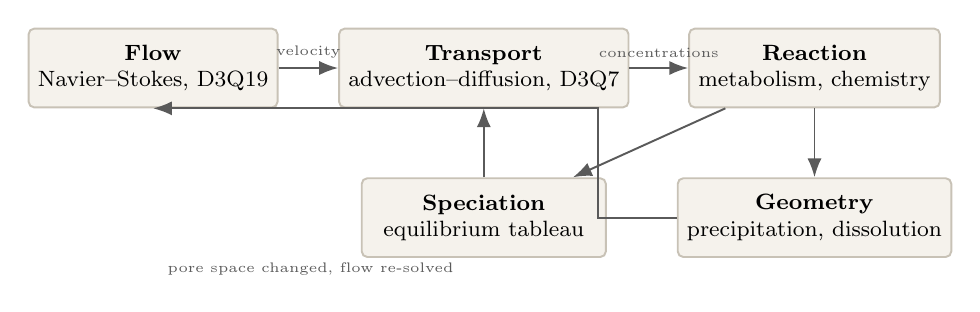
\begin{tikzpicture}[
  font=\footnotesize,
  box/.style={draw=cbRule, fill=cbSand, rounded corners=2pt, minimum width=3.1cm,
              minimum height=1.0cm, align=center, line width=0.7pt},
  arr/.style={-{Latex[length=2.4mm]}, cbGrey, line width=0.7pt}]

\node[box] (flow) at (0,0) {\textbf{Flow}\\ Navier--Stokes, D3Q19};
\node[box] (tr) at (4.2,0) {\textbf{Transport}\\ advection--diffusion, D3Q7};
\node[box] (rx) at (8.4,0) {\textbf{Reaction}\\ metabolism, chemistry};
\node[box] (eq) at (4.2,-1.9) {\textbf{Speciation}\\ equilibrium tableau};
\node[box] (geo) at (8.4,-1.9) {\textbf{Geometry}\\ precipitation, dissolution};

\draw[arr] (flow) -- node[above,font=\tiny]{velocity} (tr);
\draw[arr] (tr) -- node[above,font=\tiny]{concentrations} (rx);
\draw[arr] (rx) -- (eq);
\draw[arr] (eq) -- (tr);
\draw[arr] (rx) -- (geo);
\draw[arr] (geo.west) -- ++(-1.0,0) |- (flow.south);
\node[cbGrey,font=\tiny] at (2.0,-2.55) {pore space changed, flow re-solved};
\end{tikzpicture}
\end{center}

Every box except the first two is optional and switched on from the input file.
With all of them off, CompLB3D is a flow-and-transport solver and nothing more.
That is deliberate: you should be able to turn one thing on at a time and see
what it did.

\section{What makes it different from the 2D CompLaB}

CompLB3D began as a port of CompLaB to three dimensions and grew several
capabilities the 2D code does not have.

\begin{center}
\begin{tabular}{@{}p{5.2cm}p{4.6cm}p{4.6cm}@{}}
\toprule
& \textbf{CompLaB (2D)} & \textbf{CompLB3D}\\
\midrule
Dimensions & D2Q9 / D2Q5 & D3Q19 / D3Q7\\
Biomass solvers & CA, FD, LBM & CA, FD, LBM\\
Metabolism & kinetics, FBA, surrogate & the same, plus combined types\\
Aqueous speciation & --- & equilibrium tableau\\
Abiotic kinetics & --- & separate hook\\
Precipitation & --- & volume-of-pixel pore clogging\\
Dissolution & --- & pore reopening\\
Surrogate training & not distributed & MATLAB and Python paths\\
Worked examples & 6, one problem & 15, one per capability\\
\bottomrule
\end{tabular}
\end{center}

\section{What it is not}

Being honest about this saves time.

\begin{itemize}[leftmargin=1.2em]
\item \textbf{It is not a continuum reactive transport code.} There is no
Darcy law and no representative elementary volume. If your domain is metres
across, this is the wrong tool.
\item \textbf{The speciation is ideal.} No activity corrections, no temperature
dependence, no gas phase, no redox couples, no mineral saturation indices. The
equilibrium constants you supply are conditional constants at your own ionic
strength.
\item \textbf{There is no unsaturated flow.} One fluid phase only.
\item \textbf{Rate laws are compiled in.} Changing your chemistry means editing
a C\texttt{++} header and rebuilding. This surprises people who expect an input
file to be enough.
\end{itemize}

% =====================================================================
\chapter{Installing and building}
\label{ch:install}

\section{What you need}

\begin{center}
\begin{tabular}{@{}p{3.6cm}p{2.4cm}p{8.6cm}@{}}
\toprule
\textbf{Component} & \textbf{Required?} & \textbf{Notes}\\
\midrule
C\texttt{++} compiler & yes & GCC or Clang, C\texttt{++}11 or later\\
CMake & yes & 3.10 or later\\
Palabos & yes & \textbf{version 2.3.0}. Downloaded separately.\\
MPI & recommended & on by default; turn off with \code{-DENABLE\_MPI=OFF}\\
GLPK & optional & only for flux balance analysis through GLPK\\
Python 3 + cobrapy & optional & only for flux balance analysis through COBRApy\\
ParaView & recommended & to look at the output\\
\bottomrule
\end{tabular}
\end{center}

\warn{Palabos version matters.}{CompLB3D is developed against Palabos
\textbf{v2.3.0}. Later versions change data-processor interfaces, and the code
will not compile against them without edits. Get 2.3.0.}

\section{Step 1: get Palabos}

Palabos is a lattice-Boltzmann framework and it is a separate work under its
own licence. It is not distributed with CompLB3D, partly because it is around
100\,MB and partly because bundling someone else's AGPL library inside yours
muddies the licence question for everybody downstream.

Download \code{palabos-v2.3.0} from \url{https://palabos.unige.ch/} and unpack
it somewhere permanent.

\begin{lstlisting}[style=sh]
tar xzf palabos-v2.3.0.tar.gz -C /your/path/
\end{lstlisting}

You do not have to build Palabos separately --- CompLB3D compiles the parts it
needs. But building it once on its own is worth the ten minutes, because if
something is wrong with your compiler or MPI you will find out there, in a
project with good documentation, rather than here.

\begin{lstlisting}[style=sh]
cd /your/path/palabos-v2.3.0/build
cmake ..
make
\end{lstlisting}

Warnings during that build are normal and can be ignored as long as it finishes.

\section{Step 2: get CompLB3D}

\begin{lstlisting}[style=sh]
git clone https://github.com/shahram444/CompLB3D-lattice-Boltzmann-FBA-surrogate-COBRApy-GLPK.git
cd CompLB3D-lattice-Boltzmann-FBA-surrogate-COBRApy-GLPK
\end{lstlisting}

\section{Step 3: point CMake at Palabos}

Open \file{CMakeLists.txt} and edit the five lines that name the Palabos tree.
They are around lines 85 to 93.

\begin{lstlisting}[style=sh]
include_directories("/your/path/palabos-v2.3.0/src")
include_directories("/your/path/palabos-v2.3.0/externalLibraries")
include_directories("/your/path/palabos-v2.3.0/externalLibraries/Eigen3")
file(GLOB_RECURSE PALABOS_SRC "/your/path/palabos-v2.3.0/src/*.cpp")
file(GLOB_RECURSE EXT_SRC "/your/path/palabos-v2.3.0/externalLibraries/tinyxml/*.cpp")
\end{lstlisting}

This is the single most common reason a first build fails. If CMake reports
that it cannot find Palabos headers, this is why.

\section{Step 4: build}

\begin{lstlisting}[style=sh]
mkdir build && cd build
cmake ..
make -j
\end{lstlisting}

That gives you the plain build: flow, transport, hand-written kinetics,
speciation, precipitation and dissolution. It does \emph{not} include flux
balance analysis, because that needs an optional dependency.

\subsection{Optional: flux balance analysis through GLPK}

Install GLPK first --- your package manager will have it
(\code{apt install libglpk-dev}, \code{brew install glpk},
\code{module load glpk} on a cluster). Then:

\begin{lstlisting}[style=sh]
cmake -DENABLE_GLPK=ON ..
make -j
\end{lstlisting}

\subsection{Optional: flux balance analysis through COBRApy}

This embeds a Python interpreter, so you need the Python \emph{development}
headers, not just the interpreter.

\begin{lstlisting}[style=sh]
python3 -m pip install cobrapy
cmake -DENABLE_COBRAPY=ON ..
make -j
\end{lstlisting}

\note{Both at once.}{\code{cmake -DENABLE\_GLPK=ON -DENABLE\_COBRAPY=ON ..}
builds an executable that can do either, chosen at run time from the input
file. Worth doing once so you never think about it again.}

\subsection{The build options in full}

\begin{center}
\begin{tabular}{@{}p{4.6cm}p{1.6cm}p{8.6cm}@{}}
\toprule
\textbf{Option} & \textbf{Default} & \textbf{Effect}\\
\midrule
\code{ENABLE\_MPI} & ON & parallel build. Turn off for a single-core debug build.\\
\code{ENABLE\_GLPK} & OFF & links GLPK; enables \code{reaction\_type glpk}\\
\code{ENABLE\_COBRAPY} & OFF & embeds Python; enables \code{reaction\_type cobrapy}\\
\code{FBA\_BULK\_ONLY} & OFF & restricts the FBA processors to the bulk domain. An optimisation; leave it off until you have a reason.\\
\bottomrule
\end{tabular}
\end{center}

\section{Step 5: check the build}

The fastest confidence check is the example suite, which ships with the code.

\begin{lstlisting}[style=sh]
python3 examples/makeGeometry.py
python3 examples/makeExamples.py
python3 examples/validateExamples.py .
\end{lstlisting}

The last command checks the fifteen examples structurally --- tag names, vector
lengths, model file dimensions --- and compiles their kinetics headers. It
takes about a second and should end with:

\begin{lstlisting}[style=sh]
15 case(s) checked, 0 failed, 0 note(s).
\end{lstlisting}

Then run them:

\begin{lstlisting}[style=sh]
./examples/runAllExamples.sh .
\end{lstlisting}

\section{When the build fails}

\begin{center}
\begin{tabular}{@{}p{6.2cm}p{8.6cm}@{}}
\toprule
\textbf{Message} & \textbf{Cause and fix}\\
\midrule
\code{Cannot find palabos3D.h} & The paths in \file{CMakeLists.txt} are wrong. Step 3.\\
\code{ENABLE\_GLPK is ON but GLPK was not found} & Install \code{libglpk-dev}, or drop the flag.\\
\code{ENABLE\_COBRAPY is ON but the Python development headers were not found} & You have Python but not \code{python3-dev}. Install it.\\
undefined reference to \code{MPI\_*} & Building with MPI but linking without it. Load the same MPI module you configured with, and delete \file{build/} before reconfiguring.\\
errors inside Palabos headers & Almost always the wrong Palabos version. Check it is 2.3.0.\\
\code{defineKinetics.hh: C[94] out of range} & You are compiling a kinetics header written for different chemistry. Chapter~\ref{ch:ownkinetics}.\\
\bottomrule
\end{tabular}
\end{center}

\warn{Delete \file{build/} when you change configuration.}{CMake caches its
options. Switching \code{ENABLE\_GLPK} on and off without clearing the cache
produces builds that link the wrong things and fail in confusing ways.}

% =====================================================================
\chapter{Your first simulation}
\label{ch:first}

We will run example 01. It is the smallest thing that exercises both solvers:
water driven through a channel, and a dissolved tracer that rides along and
reacts with nothing.

\section{Run it}

\begin{lstlisting}[style=sh]
# from the top of the CompLB3D tree
cp examples/01_flow_only/defineKinetics.hh        .
cp examples/01_flow_only/defineAbioticKinetics.hh .
cd build && make -j && cd ..

mkdir -p run01 && cd run01
cp ../examples/01_flow_only/CompLaB.xml .
cp -r ../examples/01_flow_only/input .
mkdir -p output
../build/complab
\end{lstlisting}

\warn{Why the two \file{.hh} files get copied.}{CompLaB compiles its rate laws
in. \file{defineKinetics.hh} and \file{defineAbioticKinetics.hh} are
\code{\#include}d, not read at run time, so a case with different chemistry
needs a different binary. This catches everyone once. See
Chapter~\ref{ch:ownkinetics}.}

\note{\file{CompLaB.xml} is read by that exact name}{from the current working
directory. Not from the executable's directory, not from a path you pass on the
command line. Run the code from the folder that holds the input file.}

\section{What you should see}

The run prints a long banner at start-up. It is worth reading, because most
input mistakes are visible in it. The parts that matter:

\begin{lstlisting}[style=sh]
[OK] XML configuration loaded and validated

  domain          : 24 x 24 x 6   (3456 voxels)
  substrates      : 1
  microbes        : 0             (abiotic mode)
  ...
  [IMMOBILE] immobile (solid/precipitate) substrates: 0 of 1
\end{lstlisting}

then the flow solver converging, then the transport steps. At the end you have
a folder of \file{.vti} files in \file{output/}.

\section{Reading the run}

Three things are worth checking on every run you ever do.

\subsection{Did the flow converge?}

The Navier--Stokes solver iterates until the velocity field stops changing by
more than \tg{ns\_converge\_iT1}, or until \tg{ns\_max\_iT1} steps. If it hits
the iteration cap instead of the tolerance, your flow field is not converged
and everything downstream inherits that.

\subsection{Are there \code{[NEG!]} warnings?}

A negative concentration is not physical. It means a reaction removed more of
something than was there, which usually means the time step is too long for the
rate you specified. One or two at start-up while fields settle is tolerable;
a stream of them is a real problem. Chapter~\ref{ch:errors}.

\subsection{Does the answer depend on \textit{z}?}

Every shipped example is 24\,$\times$\,24\,$\times$\,6 with $z$ periodic and
the geometry extruded through the depth. That makes them quasi-2D on purpose:
every $z$-plane sees identical conditions, so the answer \emph{must not} depend
on $z$. If it does, something is wrong with the setup, not with the physics.
It is a free check and it costs nothing to look.

\section{Looking at the output}

CompLB3D writes VTK ImageData (\file{.vti}) files, one per field per save
interval. Open them in ParaView:

\begin{enumerate}[leftmargin=1.4em]
\item \textbf{File $\rightarrow$ Open}, select the numbered group
      (ParaView collapses \file{subsLattice0\_0000500.vti} and friends into one
      entry), and hit Apply.
\item Set the \textbf{Coloring} dropdown to the field you want.
\item Use \textbf{Slice} to cut through the domain; the raw view of a 3D block
      shows you only its outer surface.
\end{enumerate}

\note{The \file{.vti} files use unit spacing.}{ParaView therefore shows lattice
coordinates, not micrometres. Multiply by \tg{dx} if you need physical
distance. This is a known wart, not a setting.}

\section{What to try next}

Change one thing and rerun. Good first experiments:

\begin{center}
\begin{tabular}{@{}p{5.0cm}p{9.8cm}@{}}
\toprule
\textbf{Change} & \textbf{What should happen}\\
\midrule
\tg{Peclet} from 1 to 0 & flow switches off; the tracer profile becomes a straight line. This is example 02.\\
\tg{Peclet} from 1 to 10 & advection dominates; the tracer front sharpens and moves faster.\\
\tg{delta\_P} up & higher velocity, and the flow solver takes longer to converge.\\
\tg{nz} from 6 to 12 & the answer must not change. If it does, tell us.\\
\bottomrule
\end{tabular}
\end{center}

% =====================================================================
\chapter{The input file}
\label{ch:xml}

Everything about a run is in \file{CompLaB.xml}. This chapter walks through its
structure. Chapter~\ref{ch:reference} is the exhaustive tag list; this one is
the map.

\section{The six blocks}

\begin{center}
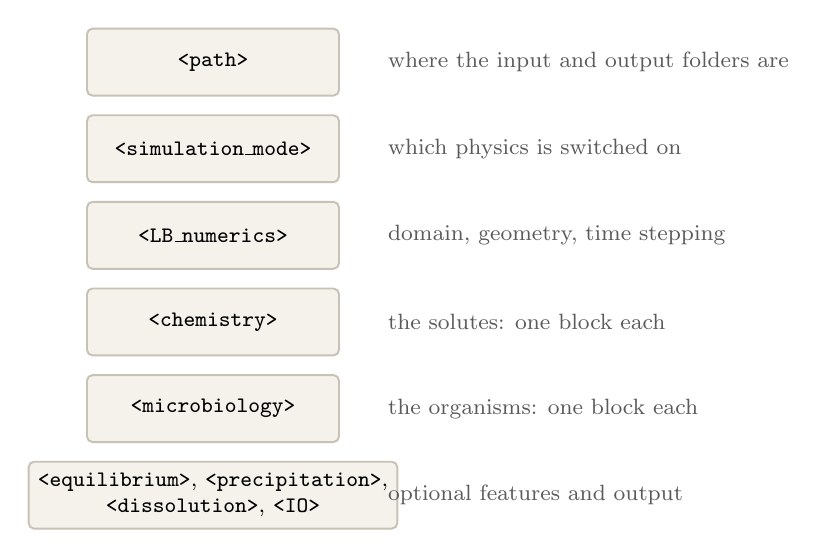
\begin{tikzpicture}[font=\footnotesize,
  b/.style={draw=cbRule,fill=cbSand,line width=0.7pt,minimum width=3.2cm,
            minimum height=0.85cm,align=center,rounded corners=2pt}]
\node[b] (p)  at (0,0)    {\texttt{<path>}};
\node[b] (s)  at (0,-1.1) {\texttt{<simulation\_mode>}};
\node[b] (l)  at (0,-2.2) {\texttt{<LB\_numerics>}};
\node[b] (c)  at (0,-3.3) {\texttt{<chemistry>}};
\node[b] (m)  at (0,-4.4) {\texttt{<microbiology>}};
\node[b] (o)  at (0,-5.5) {\texttt{<equilibrium>}, \texttt{<precipitation>},\\ \texttt{<dissolution>}, \texttt{<IO>}};

\node[anchor=west,cbGrey] at (2.1,0)    {where the input and output folders are};
\node[anchor=west,cbGrey] at (2.1,-1.1) {which physics is switched on};
\node[anchor=west,cbGrey] at (2.1,-2.2) {domain, geometry, time stepping};
\node[anchor=west,cbGrey] at (2.1,-3.3) {the solutes: one block each};
\node[anchor=west,cbGrey] at (2.1,-4.4) {the organisms: one block each};
\node[anchor=west,cbGrey] at (2.1,-5.5) {optional features and output};
\end{tikzpicture}
\end{center}

\section{\tg{simulation\_mode}: the master switches}

This block decides which physics runs at all. Everything in it is a
\code{true} or \code{false}.

\begin{lstlisting}[style=xml]
<simulation_mode>
    <biotic_mode>true</biotic_mode>
    <enable_kinetics>true</enable_kinetics>
    <enable_abiotic_kinetics>false</enable_abiotic_kinetics>
    <enable_fba_glpk>false</enable_fba_glpk>
    <enable_fba_cobrapy>false</enable_fba_cobrapy>
    <enable_surrogate>false</enable_surrogate>
</simulation_mode>
\end{lstlisting}

\tg{biotic\_mode} is the big one: \code{false} skips the whole
\tg{microbiology} block, and CompLB3D becomes a chemistry-and-transport code.

The three metabolic switches are \emph{global}. Each microbe then chooses its
own \tg{reaction\_type}, and the two have to agree --- a microbe asking for
\code{glpk} while \tg{enable\_fba\_glpk} is \code{false} stops the run with a
message. That double gate is deliberate: it means you cannot accidentally get
different biology from the one you asked for.

\section{\tg{LB\_numerics}: domain and time}

\begin{lstlisting}[style=xml]
<domain>
    <nx>24</nx> <ny>24</ny> <nz>6</nz>
    <dx>10</dx> <unit>um</unit>
    <characteristic_length>24</characteristic_length>
    <filename>geometry.dat</filename>
    <material_numbers>
        <pore>2</pore>
        <solid>0</solid>
        <bounce_back>1</bounce_back>
        <microbe0>3</microbe0>
    </material_numbers>
</domain>
\end{lstlisting}

\tg{dx} and \tg{unit} set the physical size of one voxel; here 10\,\textmu m.
\tg{characteristic\_length} is the length scale the Reynolds and P\'eclet
numbers are built on, in voxels.

\subsection{Material numbers}
\label{sec:materials}

Every voxel in the geometry file carries an integer. The
\tg{material\_numbers} block says what those integers mean.

\begin{center}
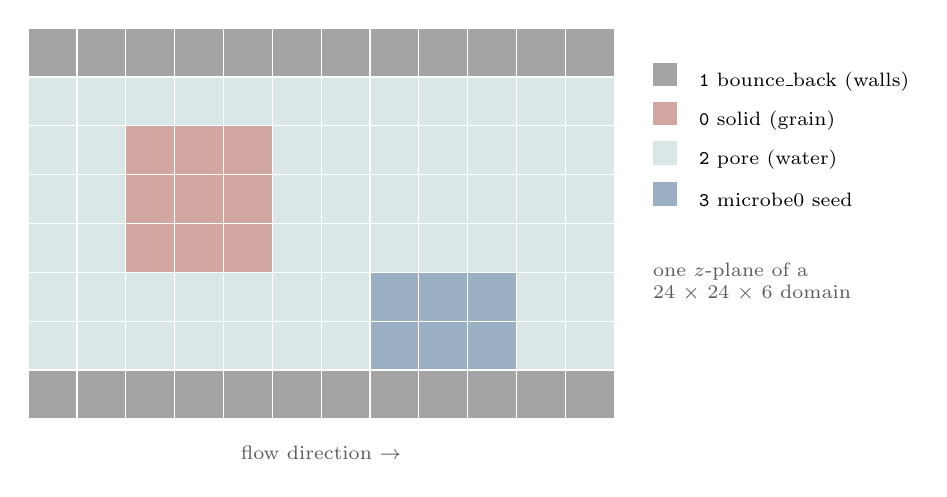
\begin{tikzpicture}[font=\footnotesize,scale=0.62]
\foreach \y in {0,...,7} \foreach \x in {0,...,11} {
  \pgfmathsetmacro{\v}{(\y==0 || \y==7) ? 1 : (((\x-3)*(\x-3)+(\y-4)*(\y-4) < 3) ? 0 : 2)}
  \pgfmathtruncatemacro{\vv}{\v}
  \ifnum\vv=1 \fill[cbGrey!55] (\x,\y) rectangle ++(1,1);\fi
  \ifnum\vv=0 \fill[cbRed!45] (\x,\y) rectangle ++(1,1);\fi
  \ifnum\vv=2 \fill[cbTeal!18] (\x,\y) rectangle ++(1,1);\fi
  \draw[white,line width=0.4pt] (\x,\y) rectangle ++(1,1);
}
\foreach \x in {7,8,9} \foreach \y in {1,2} {
  \fill[cbBlue!45] (\x,\y) rectangle ++(1,1);
  \draw[white,line width=0.4pt] (\x,\y) rectangle ++(1,1);}
\node[anchor=west,font=\scriptsize] at (12.6,7.0) {\tikz\fill[cbGrey!55](0,0)rectangle(0.3,0.3); \ \ \texttt{1} bounce\_back (walls)};
\node[anchor=west,font=\scriptsize] at (12.6,6.2) {\tikz\fill[cbRed!45](0,0)rectangle(0.3,0.3); \ \ \texttt{0} solid (grain)};
\node[anchor=west,font=\scriptsize] at (12.6,5.4) {\tikz\fill[cbTeal!18](0,0)rectangle(0.3,0.3); \ \ \texttt{2} pore (water)};
\node[anchor=west,font=\scriptsize] at (12.6,4.6) {\tikz\fill[cbBlue!45](0,0)rectangle(0.3,0.3); \ \ \texttt{3} microbe0 seed};
\node[anchor=west,font=\scriptsize,cbGrey,align=left] at (12.6,2.8)
  {one $z$-plane of a\\ 24 $\times$ 24 $\times$ 6 domain};
\node[cbGrey,font=\scriptsize] at (6,-0.7) {flow direction $\rightarrow$};
\end{tikzpicture}
\end{center}

The distinction between \code{solid} and \code{bounce\_back} matters: both stop
the flow, but \code{solid} voxels get no dynamics at all, while
\code{bounce\_back} voxels reflect the fluid. Use \code{bounce\_back} for the
domain walls and \code{solid} for grains.

A \tg{microbeN} entry does double duty: it says which voxels that organism is
seeded in, \emph{and} it marks the organism as a biofilm former rather than a
planktonic one. That has consequences described in Section~\ref{sec:biofilm}.

\subsection{The geometry file}
\label{sec:geomfile}

The geometry is a plain text file, one integer per line, $x$ fastest, then $y$,
then $z$:

\begin{lstlisting}[style=py]
for z in range(nz):
    for y in range(ny):
        for x in range(nx):
            write(mask[x][y][z])
\end{lstlisting}

So the file has exactly \code{nx*ny*nz} lines. There is no header. The examples
ship a generator, \file{examples/makeGeometry.py}, which is the easiest thing
to adapt for your own geometry.

\warn{Order, not shape.}{Nothing in the file records \code{nx}, \code{ny} or
\code{nz} --- those come from the XML. A file with the right number of values
but the wrong loop order produces a geometry that is silently transposed. If
your pore structure looks scrambled in ParaView, this is why.}

\section{\tg{chemistry}: the solutes}

One \tg{substrateN} block per solute, numbered from zero with no gaps.

\begin{lstlisting}[style=xml]
<chemistry>
    <number_of_substrates>2</number_of_substrates>

    <substrate0>
        <name_of_substrates>donor</name_of_substrates>
        <initial_concentration>0.1</initial_concentration>
        <substrate_diffusion_coefficients>
            <in_pore>5e-10</in_pore>
            <in_biofilm>5e-10</in_biofilm>
        </substrate_diffusion_coefficients>
        <left_boundary_type>Dirichlet</left_boundary_type>
        <left_boundary_condition>0.5</left_boundary_condition>
        <right_boundary_type>Neumann</right_boundary_type>
        <right_boundary_condition>0.</right_boundary_condition>
    </substrate0>
    ...
</chemistry>
\end{lstlisting}

\textbf{Dirichlet} holds the concentration at the boundary; \textbf{Neumann}
sets the flux, and \code{0} means no flux, i.e.\ a closed end.

Two optional flags are worth knowing early:

\begin{center}
\begin{tabular}{@{}p{4.0cm}p{10.8cm}@{}}
\toprule
\tg{immobile} & \code{true} means this substrate never advects or diffuses. It only receives its reaction source term. This is how minerals are represented: they must accumulate exactly where they form.\\
\tg{fix\_concentration} & a per-substrate list in \tg{chemistry}. Marks a solute as an inexhaustible reservoir: reactions read it but never draw it down.\\
\bottomrule
\end{tabular}
\end{center}

\section{\tg{microbiology}: the organisms}

One \tg{microbeN} block per organism. Two of its tags carry most of the
meaning, and they are independent of each other.

\begin{lstlisting}[style=xml]
<microbe0>
    <name_of_microbes>Bug</name_of_microbes>
    <solver_type>CA</solver_type>          <!-- how biomass MOVES -->
    <reaction_type>kinetics</reaction_type><!-- how it METABOLISES -->
    <initial_densities>1.0</initial_densities>
    <decay_coefficient>0.0</decay_coefficient>
    <viscosity_ratio_in_biofilm>0</viscosity_ratio_in_biofilm>
    <half_saturation_constants>0.05 0</half_saturation_constants>
    ...
</microbe0>
\end{lstlisting}

\subsection{Biofilm or planktonic}
\label{sec:biofilm}

An organism with a \tg{microbeN} entry under \tg{material\_numbers} is a
\emph{biofilm} former: it is seeded in those voxels and it can clog them. One
without is \emph{planktonic}: seeded uniformly through the pore space.

Three rules follow, and each stops a run when broken:

\begin{itemize}[leftmargin=1.2em]
\item \tg{viscosity\_ratio\_in\_biofilm} must be present for exactly the
biofilm organisms. The parser counts them and compares.
\item \tg{initial\_densities} must have one entry per material number the
organism is seeded in.
\item \code{solver\_type FD} is rejected for planktonic organisms.
\end{itemize}

\section{Where to look things up}

\begin{center}
\begin{tabular}{@{}p{6.4cm}p{8.4cm}@{}}
\toprule
\textbf{Question} & \textbf{Where}\\
\midrule
what does this tag do, exactly? & Chapter~\ref{ch:reference}, or the inline comments in \file{CompLaB\_reference\_template.xml}\\
what is a realistic value? & the example closest to your problem, Part~II\\
why did the run refuse to start? & Chapter~\ref{ch:errors}\\
\bottomrule
\end{tabular}
\end{center}

\note{\file{CompLaB\_reference\_template.xml}}{ships with the code and
documents every tag inline, next to a plausible value, with its units and known
limits. It is the fastest reference when you are actually editing a file.}

\part{Tutorial}

Each chapter here is built on a worked example that ships with the code, in
\file{examples/}. They are tiny --- 24\,$\times$\,24\,$\times$\,6 voxels,
seconds on a laptop --- because the point is to show what a switch does, not to
be physically interesting.

Every chapter has the same shape: what the case is, what to run, what you
should see, and what to change to learn something. Four of the cases have an
answer that does not come from this code, and those are flagged: they are the
ones worth trusting.

% =====================================================================
\chapter{Transport with no reaction}
\label{ch:transport}

\emph{Examples 01 and 02.}

\section{The point}

Before adding chemistry, be sure transport is right. These two cases have no
reactions at all, and the second has an answer you can check on paper.

\section{Example 01: flow and a tracer}

A tracer is held at 1 on the inlet face and 0 on the outlet, and reacts with
nothing. \tg{Peclet} is 1, so advection and diffusion are comparable.

\textbf{Expect:} the tracer sweeping left to right; a profile that falls
monotonically with $x$ and never rises; no \code{[NEG!]} warnings; no
dependence on $z$.

\section{Example 02: diffusion only}

The same case with \tg{Peclet} set to 0, which switches the flow solver off
entirely.

\begin{cbnote}
\textbf{\color{cbTeal}This one has a right answer.}\quad
With no flow, no reaction, one face held at 1 and the other at 0, the steady
state is the solution of $\nabla^2 C = 0$ with those boundaries --- a
\textbf{straight line} from 1 to 0 along $x$.

Plot the centreline profile. If it is straight, your diffusion coefficient,
your boundary conditions and your relaxation time are all doing what you think.
If it curves, one of them is not, and it is far easier to find out here than in
a case with biology in it.
\end{cbnote}

\section{What to change}

\begin{center}
\begin{tabular}{@{}p{4.6cm}p{10.2cm}@{}}
\toprule
\textbf{Change} & \textbf{What it tells you}\\
\midrule
\tg{Peclet} 0 $\rightarrow$ 1 $\rightarrow$ 10 & how the balance of advection and diffusion moves the front. At high P\'eclet the front sharpens and the transport solver needs smaller steps.\\
\tg{tau} away from 0.8 & the lattice-Boltzmann relaxation time. Values far from 1 are less stable; below about 0.55 the scheme misbehaves.\\
right boundary Dirichlet $\rightarrow$ Neumann & a closed end: the tracer accumulates instead of leaving.\\
\bottomrule
\end{tabular}
\end{center}

\warn{If example 02 is not straight, stop here.}{Every later chapter builds on
transport being correct. A curved profile with no reaction means something is
firing that should not be, or a boundary is not being held, and both will
corrupt everything downstream while looking plausible.}

% =====================================================================
\chapter{Abiotic kinetics}
\label{ch:abiotic}

\emph{Example 03.}

\section{The point}

Chemistry with no biology. Two reactants enter from opposite faces, meet, and
make a product:
\[
  \mathrm{A} + \mathrm{B} \longrightarrow \mathrm{C},
  \qquad \text{rate} = k\,[\mathrm{A}][\mathrm{B}]
\]

\section{Where the rate law lives}

In \file{defineAbioticKinetics.hh}, in the example's own folder. The whole
function is this:

\begin{lstlisting}[style=cpp]
void defineAbioticRxnKinetics(std::vector<double> C,
                              std::vector<double>& subsR,
                              plb::plint mask)
{
    for (std::size_t i = 0; i < subsR.size(); ++i) subsR[i] = 0.0;
    if (C.size() < 3 || subsR.size() < 3) return;
    if (mask < 2) return;              // nothing happens in solid or wall voxels

    const double A = std::max(C[0], 0.0);
    const double B = std::max(C[1], 0.0);
    const double R = k_AB * A * B;     // mol/L/s

    subsR[0] = -R;
    subsR[1] = -R;
    subsR[2] = +R;
}
\end{lstlisting}

Three things in that snippet are conventions you will reuse everywhere:

\begin{itemize}[leftmargin=1.2em]
\item \textbf{\code{C} is indexed in \file{CompLaB.xml} order.} \code{C[0]} is
\tg{substrate0}. There is no lookup by name.
\item \textbf{\code{subsR} is a rate, per second}, positive for produced and
negative for consumed. The solver multiplies by the time step.
\item \textbf{\code{std::max(x, 0.0)}} floors the tiny negative values the
lattice-Boltzmann solver can produce near steep fronts. Without it a rate law
can amplify numerical noise into a real instability.
\end{itemize}

\section{What you should see}

A peak in C near the middle, with A and B drawn down around it. With
\tg{Peclet} at 0 the front is stationary; turn the flow on and it moves
downstream.

\begin{cbnote}
\textbf{\color{cbTeal}This one has a right answer too.}\quad
One A plus one B makes exactly one C, so summed over the domain
\[
  \Delta[\mathrm{A}] + \Delta[\mathrm{C}] = 0
  \qquad\text{and}\qquad
  \Delta[\mathrm{B}] + \Delta[\mathrm{C}] = 0
\]
at every step. Any drift in those sums is a bug, not chemistry.
\end{cbnote}

% =====================================================================
\chapter{Aqueous speciation}
\label{ch:equilibrium}

\emph{Example 04.}

\section{The point}

Some chemistry is fast enough to treat as instantaneous equilibrium rather than
as a rate. CompLB3D solves a components-and-species tableau in every pore
voxel, at every step.

The example uses the smallest tableau that is still real chemistry: the
carbonate system, four species over two components.

\begin{center}
\begin{tabular}{@{}lccl@{}}
\toprule
\textbf{species} & \textbf{HCO$_3$} & \textbf{H} & \textbf{log\,K}\\
\midrule
HCO$_3$ \emph{(component)}  & 1 & 0 & 0\\
H \emph{(component)}        & 0 & 1 & 0\\
CO$_3$                      & 1 & $-1$ & $-10.33$\\
H$_2$CO$_3$                 & 1 & 1 & $6.35$\\
\bottomrule
\end{tabular}
\end{center}

In XML:

\begin{lstlisting}[style=xml]
<equilibrium>
    <enabled>true</enabled>
    <components>HCO3 H</components>
    <stoichiometry>
        <species0>1  0</species0>
        <species1>0  1</species1>
        <species2>1 -1</species2>
        <species3>1  1</species3>
    </stoichiometry>
    <logK>
        <species0>0.</species0>     <species1>0.</species1>
        <species2>-10.33</species2> <species3>6.35</species3>
    </logK>
</equilibrium>
\end{lstlisting}

\section{The rules of the tableau}

\begin{itemize}[leftmargin=1.2em]
\item \tg{components} names master species, and those names must match
\tg{name\_of\_substrates} exactly.
\item Each \tg{speciesN} row has one number per component, and \code{N} is the
substrate index.
\item A component's own row is the identity row with log\,K of 0.
\item \textbf{A row of zeros means the solver ignores that species.} That is
how minerals and biomass stay out of the tableau while still being substrates.
\end{itemize}

\section{What you should see}

The banner reports the tableau it parsed --- 2 components, 4 species. Acid
enters from the left, so H$_2$CO$_3$ should dominate near the inlet and CO$_3$
away from it.

\begin{cbnote}
\textbf{\color{cbTeal}Check the totals.}\quad
Total carbonate, summed over HCO$_3$, CO$_3$ and H$_2$CO$_3$, must change only
through transport. Speciation moves mass \emph{between} species; it never
creates or destroys a component.
\end{cbnote}

\warn{This is the expensive part.}{Speciation costs more than everything else
in the code combined. Even on 3456 voxels you will see it in the step time.
Leave it off until you need it, and if you do need it, expect the equilibrium
solve to dominate your budget.}

\section{Known limits, stated plainly}

Activities are ideal --- no Debye--H\"uckel or Davies correction. There is no
temperature dependence, no gas phase, no redox couple and no mineral saturation
index. The log\,K values you supply are therefore conditional constants at your
own ionic strength and 25\,\textdegree C. Say so in your methods section.

% =====================================================================
\chapter{Biomass and the three solvers}
\label{ch:biomass}

\emph{Examples 05, 06 and 07 --- the same case, one line different.}

\section{The point}

Biomass has to go somewhere when a colony grows. CompLB3D offers three ways of
moving it, chosen per organism with \tg{solver\_type}. Examples 05 to 07 are
identical apart from that one tag, so running all three shows you exactly what
the choice costs.

\section{The three}

\begin{center}
\begin{tabular}{@{}p{1.5cm}p{6.2cm}p{6.9cm}@{}}
\toprule
& \textbf{How it moves biomass} & \textbf{Use it when}\\
\midrule
\textbf{CA} & cellular automaton: biomass over the maximum density spills into neighbouring voxels & you want a biofilm that spreads by pushing, which is how biofilms actually grow\\
\textbf{FD} & finite difference: biomass diffuses with its own coefficient & you want smooth spreading and a diffusivity you can justify\\
\textbf{LBM} & biomass gets its own advection--diffusion lattice & biomass genuinely moves with the flow\\
\bottomrule
\end{tabular}
\end{center}

\begin{center}
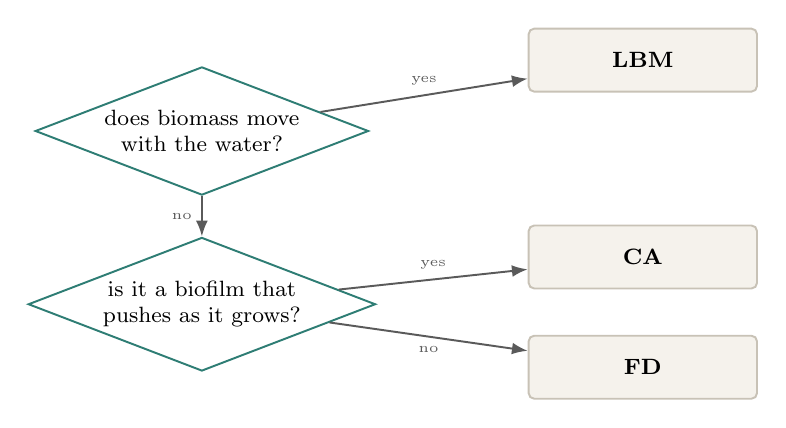
\begin{tikzpicture}[font=\footnotesize,
  n/.style={draw=cbRule,fill=cbSand,rounded corners=2pt,minimum width=2.9cm,
            minimum height=0.8cm,align=center,line width=0.7pt},
  d/.style={draw=cbTeal,fill=white,diamond,aspect=2.6,inner sep=1.5pt,
            align=center,line width=0.7pt},
  a/.style={-{Latex[length=2mm]},cbGrey,line width=0.7pt}]
\node[d] (q1) at (0,0) {does biomass move\\ with the water?};
\node[n] (lbm) at (5.6,0.9) {\textbf{LBM}};
\node[d] (q2) at (0,-2.2) {is it a biofilm that\\ pushes as it grows?};
\node[n] (ca) at (5.6,-1.6) {\textbf{CA}};
\node[n] (fd) at (5.6,-3.0) {\textbf{FD}};
\draw[a] (q1) -- node[above,font=\tiny]{yes} (lbm);
\draw[a] (q1) -- node[left,font=\tiny]{no} (q2);
\draw[a] (q2) -- node[above,font=\tiny]{yes} (ca);
\draw[a] (q2) -- node[below,font=\tiny]{no} (fd);
\end{tikzpicture}
\end{center}

\section{What each one demands of the input file}

\begin{center}
\begin{tabular}{@{}p{1.4cm}p{13.4cm}@{}}
\toprule
\textbf{CA} & needs \tg{viscosity\_ratio\_in\_biofilm}, \tg{thrd\_biofilm\_fraction} and \tg{CA\_method}. \tg{CA\_method} \code{fraction} shares the excess in proportion to the space free in each neighbour.\\
\textbf{FD} & needs \tg{biomass\_diffusion\_coefficients}. \textbf{Rejected for planktonic organisms} --- it requires a \tg{microbeN} entry under \tg{material\_numbers}.\\
\textbf{LBM} & needs \tg{biomass\_diffusion\_coefficients}. Costs one extra lattice per organism, which is the most expensive of the three in memory.\\
\bottomrule
\end{tabular}
\end{center}

\section{The rate law}

\file{defineKinetics.hh} in these folders implements Monod growth:
\[
  \text{growth} = \mu_{\max}\,\frac{S}{K_s+S}\,B,
  \qquad
  \frac{dS}{dt} = -\frac{\text{growth}}{Y},
  \qquad
  \frac{dB}{dt} = \text{growth} - k_d B
\]

\warn{\tg{half\_saturation\_constants} in the XML does not drive this.}{That
tag feeds the flux balance and surrogate paths, which build their own uptake
bounds from it. A hand-written kinetics file takes its parameters from its own
table, in the header, next to the equation that uses them. If you change $K_s$
in the XML and nothing happens, this is why.}

\section{What you should see}

Biomass rising from the seeded patch and then levelling off as growth and decay
balance. The donor drawn down around the colony and replenished from the
boundary. A product plume spreading from the colony. No \code{[NEG!]} warnings.

Run 05, 06 and 07 and compare: the biomass \emph{totals} should be close, the
spatial \emph{patterns} different. That is the honest way to see what the
solver choice actually buys you.

% =====================================================================
\chapter{More than one organism}
\label{ch:twomicrobes}

\emph{Example 08.}

\section{The point}

\tg{solver\_type} and \tg{reaction\_type} are per organism, not global. Example
08 has two microbes on opposite walls sharing one donor, one using the cellular
automaton and the other lattice Boltzmann, in the same run.

They differ in kinetics too: Bug1 has the higher $\mu_{\max}$ and the higher
$K_s$; Bug2 the reverse. So Bug1 wins where the donor is plentiful and Bug2
where it is scarce --- the classic $r$ versus $K$ trade-off. Bug1 sits nearer
the inlet, so it should end up ahead.

\section{What you should see}

Both populations growing, then their \emph{ratio} going flat. A donor shadow
between the two colonies.

\section{What to change}

Swap the two \tg{solver\_type} lines and rerun. The converged ratio should
barely move: the solver decides how biomass spreads, not how much of it there
is. If it moves a lot, that is worth understanding before you trust either
solver on a real problem.

% =====================================================================
\chapter{Flux balance analysis}
\label{ch:fba}

\emph{Examples 09 and 10.}

\section{The point}

Instead of writing a rate law, hand the organism a genome-scale metabolic model
and let a linear program work out how fast it can grow on what is locally
available. CompLB3D solves that program in every voxel, at every step.

\section{The toy model, solved by hand}

Example 09 uses a model small enough to check on paper --- three metabolites,
four reactions:

\begin{center}
\begin{tabular}{@{}clll@{}}
\toprule
\textbf{index} & \textbf{reaction} & \textbf{written as} & \textbf{meaning}\\
\midrule
0 & EX\_S & S$_c$ $\rightarrow$ & negative flux imports the donor\\
1 & EX\_O & O$_c$ $\rightarrow$ & negative flux imports the acceptor\\
2 & EX\_P & P$_c$ $\rightarrow$ & positive flux exports the product\\
3 & BIO   & S$_c$ + 0.5\,O$_c$ $\rightarrow$ P$_c$ & the objective\\
\bottomrule
\end{tabular}
\end{center}

Steady state forces $v_0 = -v_3$ and $v_1 = -\tfrac12 v_3$, so with uptake
bounds $V_S$ and $V_O$:

\begin{cbnote}
\[
  \boxed{\ \text{growth} \;=\; \min\!\left(V_S,\; 2\,V_O\right)\ }
  \qquad\text{where}\qquad
  V = V_{\max}\,\frac{C}{K_c + C}
\]
With \code{fba\_maximum\_uptake\_flux} of 10 and 4, and both concentrations
well above their half-saturation constants, $V_S \to 10$ and $2V_O \to 8$: the
acceptor limits, and growth should settle near \textbf{8\,mmol/gDW/h}.

That number comes from the stoichiometry, not from this code. It is the
strongest check in the suite.
\end{cbnote}

Change \tg{fba\_maximum\_uptake\_flux} to \code{4. 10. 0.} and the donor limits
instead, so growth should settle near 4. One line, a second independent check.

\section{How a voxel gets its answer}

\begin{center}
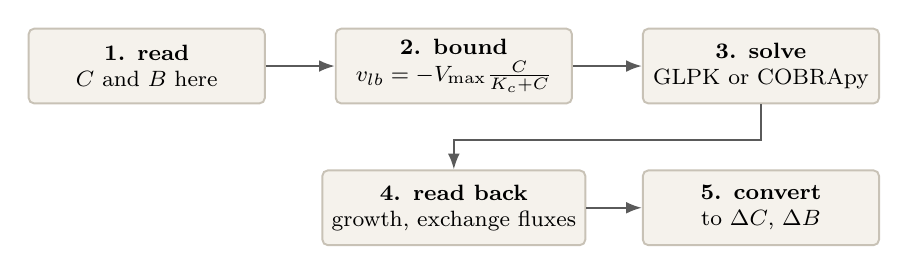
\begin{tikzpicture}[font=\footnotesize,
  s/.style={draw=cbRule,fill=cbSand,rounded corners=2pt,minimum width=3.0cm,
            minimum height=0.95cm,align=center,line width=0.7pt},
  a/.style={-{Latex[length=2mm]},cbGrey,line width=0.7pt}]
\node[s] (r) at (0,0) {\textbf{1. read}\\ $C$ and $B$ here};
\node[s] (b) at (3.9,0) {\textbf{2. bound}\\ $v_{lb}=-V_{\max}\frac{C}{K_c+C}$};
\node[s] (l) at (7.8,0) {\textbf{3. solve}\\ GLPK or COBRApy};
\node[s] (u) at (3.9,-1.8) {\textbf{4. read back}\\ growth, exchange fluxes};
\node[s] (c) at (7.8,-1.8) {\textbf{5. convert}\\ to $\Delta C$, $\Delta B$};
\draw[a] (r) -- (b);
\draw[a] (b) -- (l);
\draw[a] (l.south) -- ++(0,-0.45) -| (u.north);
\draw[a] (u) -- (c);
\end{tikzpicture}
\end{center}

Steps 1, 2, 4 and 5 are identical for GLPK and COBRApy. Only step 3 differs.

\section{GLPK or COBRApy}

\begin{center}
\begin{tabular}{@{}p{2.2cm}p{6.2cm}p{6.2cm}@{}}
\toprule
& \textbf{GLPK} & \textbf{COBRApy}\\
\midrule
how it works & a persistent \code{glp\_prob}; per voxel it only resets column bounds and re-solves from the previous basis & rebuilds the problem through optlang on every \code{optimize()} call, across a Python boundary\\
speed & the fast path & one to two orders of magnitude slower per voxel\\
needs & \code{-DENABLE\_GLPK=ON} & \code{-DENABLE\_COBRAPY=ON}, cobrapy installed, and \file{src/complab3d\_cobrapy.py} present at run time\\
\bottomrule
\end{tabular}
\end{center}

\warn{COBRApy does not read SBML.}{Both solvers eat the same
\file{*\_rGEM\_c.xml} matrix file produced by \file{extractMM.py}. COBRApy
rebuilds a \code{cobra.Model} in memory from that matrix, with anonymous
numbered reactions --- no gene names, no annotations. Its value here is as an
independent second opinion, not as a richer interface.}

\section{Getting your own model in}

\file{extractMM.py} converts a genome-scale model into the matrix file the
solvers read.

\begin{lstlisting}[style=sh]
python3 extractMM.py iAF987.xml -o input/geobacter.xml
python3 extractMM.py iJO1366.mat -o input/ecoli.xml     # COBRA Toolbox .mat
python3 extractMM.py model.json  -o input/model.xml
\end{lstlisting}

Then in \file{CompLaB.xml}:

\begin{lstlisting}[style=xml]
<model_filename>geobacter</model_filename>          <!-- no .xml -->
<exchange_reaction_indices>6 55 418 -1</exchange_reaction_indices>
<fba_maximum_uptake_flux>15. 25. 8. 0.</fba_maximum_uptake_flux>
<substrate_lower_bounds>-15. -25. -8. 0.</substrate_lower_bounds>
<substrate_upper_bounds>60. 60. 60. 0.</substrate_upper_bounds>
<objective_direction>maximize</objective_direction>
<biomass_molar_mass>24.6</biomass_molar_mass>
\end{lstlisting}

\tg{exchange\_reaction\_indices} maps each substrate, in XML order, onto the
reaction in \emph{that organism's} model that exchanges it. Use \code{-1} for a
substrate the organism does not exchange --- a single \code{-1} is what makes a
mutualism obligate.

\note{\tg{biomass\_molar\_mass}}{converts CompLB3D's molar biomass into the
gDW a metabolic model expects; 24.6\,g/mol is the generic
CH$_{1.8}$O$_{0.5}$N$_{0.2}$ formula weight. If your biomass is already in
gDW/L, set it to 1.}

\section{What you should see}

The model loading with its metabolite and reaction counts. The metabolic
summary naming the solver and the number of microbes using it. Growth
approaching the value the stoichiometry predicts. Product accumulating at the
rate biomass is made.

Run examples 09 and 10 and compare. They receive an identical linear program
and share nothing else, so agreement is strong evidence the coupling is right
and disagreement localises the bug to one of the two.

% =====================================================================
\chapter{Surrogate models}
\label{ch:surrogate}

\emph{Example 11.}

\section{The point}

Flux balance analysis is expensive: one linear program per organism, per active
voxel, per step. On a domain of a few million voxels it dominates everything.

A surrogate replaces the program with a small function fitted to it offline:
\[
  \text{uptake rates} \;\longrightarrow\; \text{growth rate}
\]
evaluated in a few hundred multiplications. Speed-ups of 100 to 1000 times are
typical.

\section{The shipped network}

\begin{center}
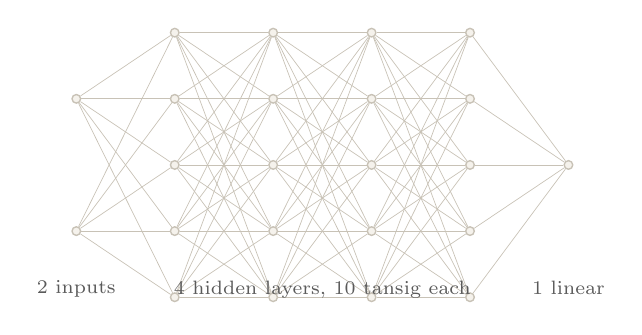
\begin{tikzpicture}[font=\scriptsize, x=1.25cm, y=0.42cm,
  nn/.style={circle,draw=cbRule,fill=cbSand,inner sep=1.1pt,line width=0.5pt}]
\foreach \i in {0,1} \node[nn] (i\i) at (0, {2-\i*4}) {};
\foreach \l in {1,2,3,4} \foreach \j in {0,...,4}
  \node[nn] (h\l\j) at (\l, {4-\j*2}) {};
\node[nn] (o) at (5,0) {};
\foreach \i in {0,1} \foreach \j in {0,...,4} \draw[cbRule,line width=0.25pt] (i\i)--(h1\j);
\foreach \l [evaluate=\l as \n using int(\l+1)] in {1,2,3}
  \foreach \j in {0,...,4} \foreach \k in {0,...,4}
    \draw[cbRule,line width=0.25pt] (h\l\j)--(h\n\k);
\foreach \j in {0,...,4} \draw[cbRule,line width=0.25pt] (h4\j)--(o);
\node[cbGrey,anchor=north] at (0,-3.2) {2 inputs};
\node[cbGrey,anchor=north] at (2.5,-3.2) {4 hidden layers, 10 tansig each};
\node[cbGrey,anchor=north] at (5,-3.2) {1 linear};
\end{tikzpicture}
\end{center}

The network shipped in \file{surrogateModel.hh} is \emph{Geobacter
metallireducens} on acetate and Fe(III), exported from MATLAB's Deep Learning
Toolbox.

\begin{cbwarn}
\textbf{\color{cbRed}A network is only valid inside the range it was trained
on.}\quad Outside it, a neural network does not fail --- it returns confident
nonsense. The shipped one was trained on

\begin{center}
\begin{tabular}{@{}lr@{ \ to \ }l@{}}
acetate  & 0.00089 & 9.998 \ mmol/gDW/h\\
Fe(III)  & 0.000035 & 0.4997 \ mmol/gDW/h\\
growth   & 0 & 0.0527 \ 1/h\\
\end{tabular}
\end{center}

Ask it for an acetate uptake of 50 and an Fe(III) uptake of 5, well outside the
box, and it cheerfully reports 0.0486\,1/h.

That is why example 11 sets \tg{fba\_maximum\_uptake\_flux} to \code{8. 0.4} ---
safely inside. Raise the second number above 0.5 and the run spends its time
extrapolating.
\end{cbwarn}

Those bounds are not documented anywhere in the network file. They were
recovered by inverting the \code{mapminmax} scaling, which is what
\file{surrogate\_training/inspectSurrogate.py} does:

\begin{lstlisting}[style=sh]
python3 surrogate_training/inspectSurrogate.py surrogateModel.hh
\end{lstlisting}

Run that on any network before trusting it, including one somebody else fitted.

\section{Fitting your own}

The shipped network encodes one organism on two substrates over one range. For
anything else you need to train your own, and Chapter~\ref{ch:trainsurrogate}
covers that end to end.

% =====================================================================
\chapter{Combining metabolism types}
\label{ch:combined}

\emph{Example 12.}

\section{The point}

A metabolic model describes what the network can do; it does not describe
everything a cell does. Maintenance is the standard example: a constant per
biomass drain that yields no growth. A plain flux balance objective omits it,
so the model over-predicts growth at low substrate.

The combined reaction types run both paths and \textbf{add} the rates:

\begin{center}
\code{glpk\_and\_kinetics} \qquad \code{cobrapy\_and\_kinetics} \qquad
\code{surrogate\_and\_kinetics}
\end{center}

\section{The sign discipline}

\begin{cbwarn}
\textbf{\color{cbRed}Do not write \code{bioR} in a kinetics file that runs
alongside FBA.}\quad Growth belongs to the metabolic path. Writing it in both
places double counts it, and the result looks plausible --- just wrong by a
factor that depends on the substrate field.

Example 12's \file{defineKinetics.hh} writes \code{subsR} only, and says so in
a comment. Copy that discipline.
\end{cbwarn}

\section{Two Vmax tags, not one}

A combined organism needs both:

\begin{center}
\begin{tabular}{@{}p{5.4cm}p{9.4cm}@{}}
\toprule
\tg{maximum\_uptake\_flux} & read by the \textbf{kinetics} path, in mol substrate per mol cells per second\\
\tg{fba\_maximum\_uptake\_flux} & read by the \textbf{metabolic} path, in mmol/gDW/h\\
\bottomrule
\end{tabular}
\end{center}

One number cannot satisfy both meanings. If you supply only the shared tag, the
metabolic layer uses it and prints a warning about the units.

\section{What you should see}

The same growth rate as example 09, because maintenance adds no biomass --- but
the donor drawn down faster, by exactly the maintenance term. Diff the two
donor profiles: the difference \emph{is} the maintenance, and it confirms the
paths are adding rather than one silently winning.

% =====================================================================
\chapter{Precipitation and dissolution}
\label{ch:precip}

\emph{Examples 13, 14 and 15.}

\section{The point}

Minerals form, fill pore space and block the flow; acid arrives and eats them
back out again. The geometry is not a fixed input --- it is a state variable.

\section{The voxel life cycle}

\begin{center}
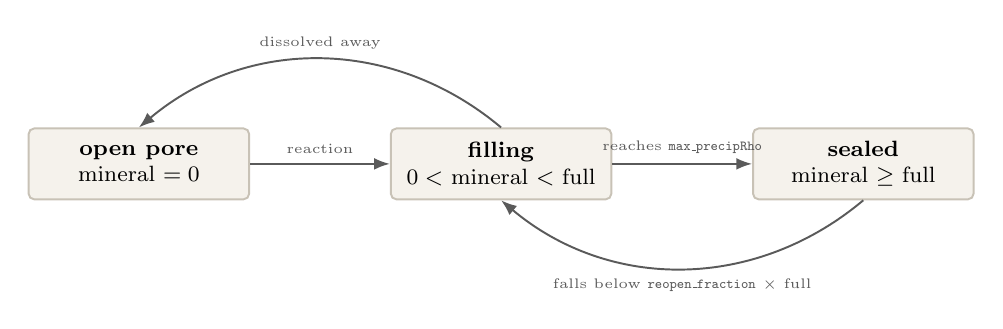
\begin{tikzpicture}[font=\footnotesize,
  st/.style={draw=cbRule,fill=cbSand,rounded corners=2pt,minimum width=2.8cm,
             minimum height=0.9cm,align=center,line width=0.7pt},
  a/.style={-{Latex[length=2mm]},cbGrey,line width=0.7pt}]
\node[st] (open) at (0,0) {\textbf{open pore}\\ mineral $=0$};
\node[st] (fill) at (4.6,0) {\textbf{filling}\\ $0<$ mineral $<$ full};
\node[st] (seal) at (9.2,0) {\textbf{sealed}\\ mineral $\ge$ full};
\draw[a] (open) -- node[above,font=\tiny]{reaction} (fill);
\draw[a] (fill) -- node[above,font=\tiny]{reaches \texttt{max\_precipRho}} (seal);
\draw[a] (seal.south) to[out=-140,in=-40] node[below,font=\tiny]
  {falls below \texttt{reopen\_fraction} $\times$ full} (fill.south);
\draw[a] (fill.north) to[out=140,in=40] node[above,font=\tiny]{dissolved away} (open.north);
\end{tikzpicture}
\end{center}

\section{Example 13: precipitation}

\[ \mathrm{Fe}^{2+} + \mathrm{HS}^- \longrightarrow \mathrm{FeS(s)} \]

Three things make this work:

\begin{enumerate}[leftmargin=1.4em]
\item The mineral substrate is \textbf{\tg{immobile}}. It never advects or
diffuses, so it accumulates exactly where it forms. A mineral that moved would
never seal anything.
\item \tg{max\_precipRho} is the mol/L of a completely full voxel, derived from
the mineral: $1000 / V_m$ with $V_m$ in cm$^3$/mol. Mackinawite is
87.91\,g/mol over 4.30\,g/cm$^3$, so $V_m = 20.44$ and
\tg{max\_precipRho} $= 48.9$.
\item \tg{surface\_only} \code{1} restricts growth to wall-adjacent voxels ---
heterogeneous nucleation, which is the physically right choice. Set it to 0 and
the mineral grows anywhere, sealing pore throats far too readily.
\end{enumerate}

\textbf{Expect:} FeS building in a band across the middle; the porosity in the
log falling in steps, one per update interval; the flow re-solved after each
conversion; and mass conserved --- every mole of FeS removes one Fe$^{2+}$ and
one HS$^-$.

\section{Example 14: dissolution}

\[ \mathrm{CaCO_3(s)} + \mathrm{H}^+ \longrightarrow \mathrm{Ca}^{2+} + \mathrm{HCO_3}^- \]

Dissolution has its own hook, \code{defineDissolutionRate()}, in the same
header. It is handed:

\begin{center}
\begin{tabular}{@{}p{2.2cm}p{12.6cm}@{}}
\toprule
\code{phaseId} & which declared phase this is, numbered from 1 in \tg{phaseN} order\\
\code{C} & the water \textbf{touching} the mineral: the open neighbours' concentrations, averaged. A solid voxel has no water of its own that moves.\\
\code{mineral} & mol/L of mineral left in this voxel\\
\bottomrule
\end{tabular}
\end{center}

and must return \code{mineralR} \textbf{negative}, plus the released solutes in
\code{subsR}, positive. Do not write the mineral's own \code{subsR} entry --- the
solver does that from \code{mineralR}.

\subsection{Why phases must be declared}

Only what appears in a \tg{phaseN} block can dissolve, and that is deliberate.
If the rule were simply ``a solid voxel with no mineral left becomes pore'',
then an inert quartz grain --- which never held any mineral --- is already below
any threshold, and your whole grain pack would dissolve on the first step.
Declaring phases makes quartz safe by construction.

\begin{lstlisting}[style=xml]
<phase0>
    <name>calcite_grain</name>
    <material_number>0</material_number>   <!-- the solid grains -->
    <substrate>2</substrate>               <!-- holds its inventory -->
    <full_density>27.1</full_density>      <!-- mol/L when full -->
    <initial_fill>27.1</initial_fill>      <!-- starts solid -->
</phase0>
\end{lstlisting}

\tg{initial\_fill} is the point of example 14: the grains \emph{start} solid
and are eaten away. Dissolution is not limited to material that precipitated
first. A precipitate phase instead uses \tg{initial\_fill} 0 and
\tg{is\_precipitate} \code{true}.

\textbf{Expect:} the acid eating into the \emph{upstream} faces first; Ca$^{2+}$
leaving downstream; porosity rising in steps, the mirror of example 13.

\section{Example 15: both at once}

Both blocks enabled, on one mineral, so a voxel can seal and later reopen.

\begin{cbnote}
\textbf{\color{cbTeal}This is what \tg{reopen\_fraction} is for.}\quad
With both directions active a voxel can sit near the threshold. A single
threshold makes it flip open and shut every update interval, and every flip
re-solves the flow. \tg{reopen\_fraction} 0.9 puts a gap between sealing at
full density and reopening below $0.9\times$ full, so it settles instead of
chattering.

Set it to 0.99 and rerun: you should see the porosity oscillate, with a flow
solve wasted on each flip. That is the failure the hysteresis prevents.
\end{cbnote}

The two rate laws are \emph{not} inverses. Precipitation is second order in the
dissolved ions; dissolution is first order in acid and in remaining mineral.
They are separate laws that happen to move the same mineral --- which is how the
code has to work, because the speciation solver computes no solubility
products and so there is no saturation state to drive a single reversible rate.

\part{Going further}

% =====================================================================
\chapter{Writing your own kinetics}
\label{ch:ownkinetics}

\section{The thing to understand first}

\begin{cbwarn}
\textbf{\color{cbRed}Rate laws are compiled in, not read from the input
file.}\quad
\file{defineKinetics.hh} and \file{defineAbioticKinetics.hh} are
\code{\#include}d into the executable. Changing your chemistry means editing a
C\texttt{++} header and rebuilding. Two problems with different chemistry need
two binaries.

This is the single most surprising thing about the code, and it is why every
example folder carries its own pair of headers and why
\file{runAllExamples.sh} rebuilds between cases.
\end{cbwarn}

\section{The two hooks}

\begin{center}
\begin{tabular}{@{}p{4.6cm}p{10.2cm}@{}}
\toprule
\code{defineRxnKinetics} & biotic. Gets the biomass vector as well as the
concentrations, and writes growth rates. Runs when \tg{enable\_kinetics} is
true, for organisms whose \tg{reaction\_type} includes kinetics.\\
\code{defineAbioticRxnKinetics} & abiotic. Concentrations only. Runs when
\tg{enable\_abiotic\_kinetics} is true.\\
\code{defineDissolutionRate} & the dissolution hook, in the abiotic file. Runs
only when \tg{dissolution} is enabled.\\
\bottomrule
\end{tabular}
\end{center}

\section{Anatomy of a biotic rate law}

\begin{lstlisting}[style=cpp]
void defineRxnKinetics(
    std::vector<double>  B,      // IN : biomass here, gDW/L, one per microbe
    std::vector<double>  C,      // IN : concentrations here, XML order
    std::vector<double>& subsR,  // OUT: dC/dt per substrate, per SECOND
    std::vector<double>& bioR,   // OUT: dB/dt per microbe,   per SECOND
    plb::plint           mask)   // IN : material number of this voxel
{
    for (std::size_t i = 0; i < subsR.size(); ++i) subsR[i] = 0.0;
    for (std::size_t i = 0; i < bioR.size();  ++i) bioR[i]  = 0.0;
    if (C.size() < 2 || subsR.size() < 2) return;   // guard: your chemistry size
    if (mask < 2) return;                           // no biology in solid/wall

    const double S = std::max(C[0], 0.0);

    for (std::size_t m = 0; m < B.size(); ++m) {
        const double Bm = std::max(B[m], 0.0);
        if (Bm <= 0.0) continue;

        const double growth = mu_max[m] * S / (Ks[m] + S) * Bm;   // gDW/L/s

        bioR[m]  += growth - kd[m] * Bm;
        subsR[0] -= growth / Y[m];
        subsR[1] += growth * fP[m];
    }
}
\end{lstlisting}

\section{The six rules}

\begin{enumerate}[leftmargin=1.4em]
\item \textbf{Indices follow \file{CompLaB.xml}.} \code{C[0]} is
\tg{substrate0}; \code{B[0]} is \tg{microbe0}. There is no lookup by name, so
reordering substrates in the XML silently changes what your rate law means.
Keep a comment naming each index at the top of the file.

\item \textbf{Everything is per second.} A rate constant published per day must
be divided by 86400.

\begin{cbwarn}
\textbf{\color{cbRed}This causes more dead runs than anything else in the
code.}\quad A rate 86400 times too large blows up on the first step; a rate
86400 times too small does nothing at all and looks like a configuration
problem. Write the unit in a comment next to every constant.
\end{cbwarn}

\item \textbf{Zero the output arrays first.} They are reused between voxels. A
rate law that returns early without zeroing leaks the previous voxel's answer
into this one.

\item \textbf{Guard on size, and match your chemistry.} The
\code{if (C.size() < 2)} line is not decoration. The shipped uranium network
guards with \code{C.size() < 14}; drop that file into a two-substrate case and
it reads past the end of the array. \file{validateExamples.py} checks this
guard against the substrate count for exactly that reason.

\item \textbf{Floor negatives.} \code{std::max(x, 0.0)} on every concentration
you read. The lattice-Boltzmann solver can produce small negative values near
steep fronts, and a rate law that squares one amplifies noise into an
instability.

\item \textbf{Never call \code{exit()}.} Under MPI it leaves the other ranks
hanging and destroys the run. Print a warning and return a safe value; a voxel
that grows at zero rate is visible in the output and recoverable.
\end{enumerate}

\section{Checking a rate law before you trust it}

Mass balance is the cheapest real test, and you can do it without Palabos.
Compile the header on its own against a stub, feed it random states, and check
the conservation you know must hold:

\begin{lstlisting}[style=cpp]
// mini driver: A + B -> C must satisfy dA + dC = 0 and dB + dC = 0
for (int trial = 0; trial < 20000; ++trial) {
    std::vector<double> C = {rnd(), rnd(), rnd()}, R(3);
    defineAbioticRxnKinetics(C, R, 2);
    assert(std::fabs(R[0] + R[2]) < 1e-12);
    assert(std::fabs(R[1] + R[2]) < 1e-12);
}
\end{lstlisting}

\file{validateExamples.py} does the compile half of this for every example; the
balance half is worth writing for your own chemistry, once.

% =====================================================================
\chapter{Training your own surrogate}
\label{ch:trainsurrogate}

The network shipped in \file{surrogateModel.hh} encodes one organism, two
substrates, one range. For anything else you fit your own. Everything for that
is in \file{surrogate\_training/}.

\section{The three steps}

\begin{center}
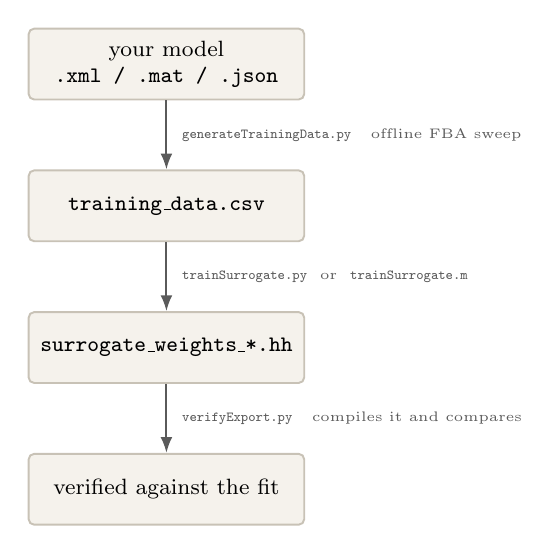
\begin{tikzpicture}[font=\footnotesize,
  s/.style={draw=cbRule,fill=cbSand,rounded corners=2pt,minimum width=3.5cm,
            minimum height=0.9cm,align=center,line width=0.7pt},
  a/.style={-{Latex[length=2mm]},cbGrey,line width=0.7pt}]
\node[s] (m) at (0,0)    {your model\\ \texttt{.xml / .mat / .json}};
\node[s] (d) at (0,-1.8) {\texttt{training\_data.csv}};
\node[s] (h) at (0,-3.6) {\texttt{surrogate\_weights\_*.hh}};
\node[s] (v) at (0,-5.4) {verified against the fit};
\draw[a] (m) -- node[right,font=\tiny,xshift=2pt]{\texttt{generateTrainingData.py} \ \ offline FBA sweep} (d);
\draw[a] (d) -- node[right,font=\tiny,xshift=2pt]{\texttt{trainSurrogate.py} \ or \ \texttt{trainSurrogate.m}} (h);
\draw[a] (h) -- node[right,font=\tiny,xshift=2pt]{\texttt{verifyExport.py} \ \ compiles it and compares} (v);
\end{tikzpicture}
\end{center}

\section{Step 1: sweep the FBA offline}

\begin{lstlisting}[style=sh]
python3 generateTrainingData.py iAF987.xml \
    --exchange EX_ac_e   --range 1e-3 10   --log \
    --exchange EX_fe3_e  --range 1e-5 0.5  --log \
    --samples 4000 --seed 1 \
    -o geobacter_training.csv
\end{lstlisting}

\subsection{Choosing the range}

\begin{cbnote}
Use the range the \textbf{simulation} will visit, not the range the organism
can tolerate. CompLB3D's uptake bound is
$V = V_{\max} C/(K_c+C)$, so the largest uptake any voxel can ever request is
$V_{\max}$ --- your \tg{fba\_maximum\_uptake\_flux}. That is the natural upper
end of the sweep. The lower end should be small but non-zero.
\end{cbnote}

Sample \textbf{logarithmically} whenever the range spans more than about one
order of magnitude. Pore-network concentrations routinely span four, and a
linear grid puts nearly all its points in the top decade --- so the fit is worst
exactly where the biology is most sensitive.

Keep to \textbf{1 to 3 inputs}. Beyond that the sample count needed for the
same accuracy grows fast and the fit stops being worth the trouble.

\section{Step 2: fit and export}

Two paths, writing byte-identical output. Use whichever you have:

\begin{center}
\begin{tabular}{@{}p{4.8cm}p{10.0cm}@{}}
\toprule
\file{trainSurrogate.m} & MATLAB, Deep Learning Toolbox, \code{trainlm}. Reconstructs how the shipped network was made.\\
\file{trainSurrogate.py} & numpy and scipy, L-BFGS-B on analytic gradients. No licence needed.\\
\bottomrule
\end{tabular}
\end{center}

\begin{lstlisting}[style=sh]
python3 trainSurrogate.py geobacter_training.csv \
    --name geobacter --microbe-id 0 \
    -o surrogate_weights_geobacter.hh
\end{lstlisting}

Both default to the shipped architecture --- 4 hidden layers of 10 tansig
neurons and a linear output, with \code{mapminmax} scaling on both ends --- so a
retrained network drops into an existing build with no other change.

\section{Step 3: verify}

\begin{lstlisting}[style=sh]
python3 verifyExport.py surrogate_weights_geobacter.hh
\end{lstlisting}

\begin{cbnote}
\textbf{\color{cbTeal}Do not skip this.}\quad An exporter that transposes a
matrix or drops a digit produces a header that compiles, runs, and is wrong,
with no independent reference to notice. So the trainer writes 512 reference
predictions next to the header, and \file{verifyExport.py} compiles the header
and checks them. It should report agreement to about $10^{-13}$ relative.
\end{cbnote}

\section{Installing it}

The generated header is namespaced, so several organisms coexist:

\begin{lstlisting}[style=cpp]
#include "surrogate_weights_geobacter.hh"
...
else if (microbeId == 0) {
    bioR[microbeId] = srgnet_geobacter::eval(Fin[microbeId]);
}
\end{lstlisting}

Then \tg{enable\_surrogate} \code{true} and
\tg{reaction\_type} \code{surrogate} in the XML.

Every generated header also carries \code{inTrainingRange()}. Call it if a run
may wander outside the box.

\section{Inspecting a network somebody else fitted}

\begin{lstlisting}[style=sh]
python3 inspectSurrogate.py surrogateModel.hh
\end{lstlisting}

The training range is not stored anywhere as such --- but \code{mapminmax} is
invertible, so it can be recovered exactly:
\[
  \text{gain} = \frac{2}{x_{\max}-x_{\min}},\quad
  \text{offset} = x_{\min}
  \qquad\Longrightarrow\qquad
  x_{\max} = \text{offset} + \frac{2}{\text{gain}}
\]

Run it before trusting any network, including the shipped one.

% =====================================================================
\chapter{Running on a cluster}
\label{ch:cluster}

\section{MPI}

MPI is on by default. Nothing in the input file changes; you launch with
\code{srun} or \code{mpirun} instead of running the binary directly.

\begin{lstlisting}[style=sh]
srun ./complab
\end{lstlisting}

Palabos decomposes the domain into blocks, one per rank, with a halo. That has
a consequence worth internalising:

\begin{cbwarn}
\textbf{\color{cbRed}More ranks is not always faster.}\quad Each rank needs
enough interior voxels to be worth the halo exchange. The shipped examples are
3456 voxels; on 36 ranks that is about 96 voxels each, nearly all of them halo,
and the run is slower than on one core. Ask for ranks in proportion to your
domain, not to what the queue will give you.
\end{cbwarn}

\section{A Slurm script}

\file{comp.sh} is a production template; \file{examples/runExamples.slurm}
submits the example suite. The parts that matter:

\begin{lstlisting}[style=sh]
#SBATCH --account=PROJECT          # required, or the job is rejected
#SBATCH --nodes=1
#SBATCH --ntasks-per-node=36       # match this to your domain size
#SBATCH --time=04:00:00

cd $SLURM_SUBMIT_DIR               # complab reads CompLaB.xml from the cwd
module purge
module load gcc openmpi            # THE SAME modules you built with
srun ./complab
\end{lstlisting}

\note{Load the same modules you built with.}{A binary built against one MPI and
launched under another fails in ways that look like your code is broken. Put
the \code{module load} line in both the build script and the run script, and
keep them identical.}

\section{Optional dependencies on a cluster}

\begin{center}
\begin{tabular}{@{}p{3.4cm}p{11.4cm}@{}}
\toprule
GLPK & \code{module load glpk}, or build it in your home directory and point \file{CMakeLists.txt} at it\\
COBRApy & needs cobrapy importable \textbf{at run time}, not just at build time, and \file{src/complab3d\_cobrapy.py} present at \tg{src\_path}. A virtualenv that is not activated in the job script is the usual failure.\\
\bottomrule
\end{tabular}
\end{center}

\section{Restarting}

Long runs should checkpoint. Set \tg{save\_CHK\_interval} to something
non-zero, and resume with:

\begin{lstlisting}[style=xml]
<read_NS_file>true</read_NS_file>
<read_ADE_file>true</read_ADE_file>
\end{lstlisting}

The flow field and the chemistry restart independently, which is useful: a
converged flow field on a fixed geometry can be reused across many chemistry
runs.

% =====================================================================
\chapter{Output and post-processing}
\label{ch:output}

\section{What gets written}

\begin{center}
\begin{tabular}{@{}p{4.2cm}p{3.0cm}p{7.4cm}@{}}
\toprule
\textbf{File} & \textbf{Format} & \textbf{Contents}\\
\midrule
\code{nsLattice*.vti} & VTK ImageData & velocity and pressure\\
\code{maskLattice*.vti} & VTK ImageData & material numbers, which change if minerals do\\
\code{subsLattice}$n$\code{*.vti} & VTK ImageData & substrate $n$\\
\code{bioLattice}$n$\code{*.vti} & VTK ImageData & microbe $n$\\
\code{*.chk} & Palabos binary & checkpoints, for restart\\
\bottomrule
\end{tabular}
\end{center}

The index and the iteration number are appended to each filename, so
\file{subsLattice0\_0000500.vti} is substrate 0 at step 500.

\section{ParaView}

\begin{enumerate}[leftmargin=1.4em]
\item \textbf{Open} the numbered group; ParaView collapses the time series into
one entry.
\item \textbf{Apply}, then set \textbf{Coloring} to the field.
\item \textbf{Slice} to see inside. The default view of a 3D block shows only
its outer surface, which for a pore network is almost useless.
\item \textbf{Threshold} on the mask field to hide solid voxels.
\end{enumerate}

\note{Unit spacing.}{The \file{.vti} files are written with spacing 1, so
ParaView shows lattice coordinates. Multiply by \tg{dx} for physical distance,
or set the spacing in ParaView's Information panel.}

\section{Getting numbers out}

For anything quantitative --- a breakthrough curve, a mass balance, a converged
biomass ratio --- read the \file{.vti} files with a script rather than reading
values off a picture.

\begin{lstlisting}[style=py]
# pip install vtk numpy
import vtk
from vtk.util.numpy_support import vtk_to_numpy

r = vtk.vtkXMLImageDataReader()
r.SetFileName("output/subsLattice0_0000500.vti")
r.Update()
img  = r.GetOutput()
dims = img.GetDimensions()
arr  = vtk_to_numpy(img.GetPointData().GetArray(0)).reshape(dims[::-1])

print("total:", arr.sum())          # for mass balance
print("mid-plane profile:", arr[dims[2]//2, dims[1]//2, :])
\end{lstlisting}

\section{The checks worth automating}

\begin{center}
\begin{tabular}{@{}p{4.2cm}p{10.6cm}@{}}
\toprule
\textbf{Check} & \textbf{Why}\\
\midrule
totals over time & mass balance. A conservative tracer's total should change only through the boundaries.\\
$z$-independence & every shipped example is quasi-2D; a $z$ dependence is a bug.\\
negative minimum & should never be below zero by more than round-off.\\
porosity & for precipitation and dissolution runs, the number that tells the story.\\
\bottomrule
\end{tabular}
\end{center}

\part{Reference}

% =====================================================================
\chapter{Every tag in CompLaB.xml}
\label{ch:reference}

This chapter lists every element the code reads, with its type, default and
units. Where a tag is mandatory only under some condition, that condition is
stated: those are the ones that stop a run.

\note{The file that documents itself.}{\file{CompLaB\_reference\_template.xml}
ships with the code and carries all of this as inline comments, next to a
plausible value. When you are actually editing a file, that is faster than this
chapter.}

\section{\tg{path}}

\begin{longtable}{@{}p{3.2cm}p{1.6cm}p{2.0cm}p{7.6cm}@{}}
\toprule
\textbf{Tag} & \textbf{Type} & \textbf{Default} & \textbf{Meaning}\\
\midrule\endhead
\tg{src\_path} & string & \code{src} & where \file{complab3d\_cobrapy.py} is found at run time. Only used by the COBRApy path, but it is imported by name, so the file must be there.\\
\tg{input\_path} & string & \code{input} & geometry and metabolic model files\\
\tg{output\_path} & string & \code{output} & VTK and checkpoint files. Must exist; the code does not create it.\\
\bottomrule
\end{longtable}

\section{\tg{simulation\_mode}}

\begin{longtable}{@{}p{4.6cm}p{1.4cm}p{1.6cm}p{6.8cm}@{}}
\toprule
\textbf{Tag} & \textbf{Type} & \textbf{Default} & \textbf{Meaning}\\
\midrule\endhead
\tg{biotic\_mode} & bool & \code{true} & \code{false} skips the whole \tg{microbiology} block and runs pure chemistry\\
\tg{enable\_kinetics} & bool & \code{true} & run \file{defineKinetics.hh}\\
\tg{enable\_abiotic\_kinetics} & bool & \code{false} & run \file{defineAbioticKinetics.hh}\\
\tg{enable\_fba\_glpk} & bool & \code{false} & global switch for GLPK. Needs \code{-DENABLE\_GLPK=ON}.\\
\tg{enable\_fba\_cobrapy} & bool & \code{false} & global switch for COBRApy. Needs \code{-DENABLE\_COBRAPY=ON}.\\
\tg{enable\_surrogate} & bool & \code{false} & global switch for the surrogate network\\
\tg{fba\_concentration\_basis} & string & \code{free} & \code{free} or \code{total}. With speciation on, whether the uptake bound is built from the free ion or the total.\\
\tg{glpk\_lpsolver} & int & 1 & 1 simplex, 2 interior point. GLPK only.\\
\tg{glpk\_save\_problem} & bool & \code{false} & dump the LP of the first solve, for debugging\\
\tg{enable\_validation\_diagnostics} & bool & \code{false} & extra consistency printing at start-up. Worth switching on while setting a case up.\\
\bottomrule
\end{longtable}

\warn{The two gates must agree.}{A microbe asking for \code{glpk} while
\tg{enable\_fba\_glpk} is \code{false} terminates the run with a message. So
does a switch that is on in an executable built without the dependency. That is
deliberate: you cannot silently get different biology from the one you asked
for.}

\section{\tg{LB\_numerics}}

\subsection{\tg{domain}}

\begin{longtable}{@{}p{4.2cm}p{1.6cm}p{1.6cm}p{7.0cm}@{}}
\toprule
\textbf{Tag} & \textbf{Type} & \textbf{Default} & \textbf{Meaning}\\
\midrule\endhead
\tg{nx} \tg{ny} \tg{nz} & int & --- & domain size in voxels. Mandatory.\\
\tg{dx} & float & --- & voxel size, in \tg{unit}\\
\tg{unit} & string & \code{um} & \code{m}, \code{mm} or \code{um}\\
\tg{characteristic\_length} & float & \code{ny} & length scale for the P\'eclet and Reynolds numbers, in voxels\\
\tg{filename} & string & --- & geometry file, inside \tg{input\_path}\\
\bottomrule
\end{longtable}

\subsection{\tg{material\_numbers}}

\begin{longtable}{@{}p{3.4cm}p{2.4cm}p{1.4cm}p{7.6cm}@{}}
\toprule
\textbf{Tag} & \textbf{Type} & \textbf{Default} & \textbf{Meaning}\\
\midrule\endhead
\tg{pore} & int list & 2 & open fluid. A list, so several codes can be pore.\\
\tg{solid} & int & 0 & no dynamics at all\\
\tg{bounce\_back} & int & 1 & no-slip wall\\
\tg{microbe}$n$ & int list & --- & voxels where microbe $n$ is seeded. Its presence also marks the organism as a biofilm former.\\
\bottomrule
\end{longtable}

\subsection{Flow and time stepping}

\begin{longtable}{@{}p{4.0cm}p{1.4cm}p{1.8cm}p{7.2cm}@{}}
\toprule
\textbf{Tag} & \textbf{Type} & \textbf{Default} & \textbf{Meaning}\\
\midrule\endhead
\tg{delta\_P} & float & 0 & pressure drop driving the flow, lattice units\\
\tg{Peclet} & float & 0 & 0 means no flow: pure diffusion, and the Navier--Stokes solver never runs\\
\tg{tau} & float & 0.8 & lattice-Boltzmann relaxation time. Values below about 0.55 are unstable.\\
\tg{track\_performance} & bool & \code{false} & timing output. Suppresses all VTI and checkpoint writing.\\
\tg{ns\_max\_iT1} & int & 100000 & flow solver step cap, first solve\\
\tg{ns\_max\_iT2} & int & 100000 & the same for later re-solves, after the geometry changes\\
\tg{ns\_converge\_iT1} & float & 1e-8 & ``flow is steady'' tolerance, first solve\\
\tg{ns\_converge\_iT2} & float & 1e-6 & the same, later\\
\tg{ns\_update\_interval} & int & 1 & re-solve the flow every $N$ reaction steps\\
\tg{ade\_update\_interval} & int & 1 & apply reactions every $N$ transport steps\\
\tg{ade\_max\_iT} & int & 1e7 & reaction and transport steps to run\\
\tg{ade\_converge\_iT} & float & 1e-8 & stop early if the chemistry stops changing\\
\bottomrule
\end{longtable}

\section{\tg{chemistry}}

\begin{longtable}{@{}p{4.6cm}p{1.8cm}p{1.4cm}p{6.6cm}@{}}
\toprule
\textbf{Tag} & \textbf{Type} & \textbf{Default} & \textbf{Meaning}\\
\midrule\endhead
\tg{number\_of\_substrates} & int & --- & must equal the number of \tg{substrateN} blocks\\
\tg{fix\_concentration} & bool list & all false & one per substrate. Marks an inexhaustible reservoir: read but never drawn down. Accepts \code{yes}/\code{no} and \code{1}/\code{0}.\\
\tg{fix\_lower\_bounds} & bool list & all false & one per substrate. Clamps the FBA uptake bound to what is locally present.\\
\bottomrule
\end{longtable}

\subsection{Each \tg{substrateN}}

\begin{longtable}{@{}p{5.4cm}p{1.4cm}p{1.4cm}p{6.2cm}@{}}
\toprule
\textbf{Tag} & \textbf{Type} & \textbf{Default} & \textbf{Meaning}\\
\midrule\endhead
\tg{name\_of\_substrates} & string & --- & used in output and to match \tg{components}\\
\tg{initial\_concentration} & float & 0 & mol/L everywhere at $t=0$\\
\tg{substrate\_diffusion\_} \tg{coefficients}/\tg{in\_pore} & float & 1e-9 & m$^2$/s in open water\\
\quad \dots/\tg{in\_biofilm} & float & 2e-10 & m$^2$/s inside biofilm\\
\tg{immobile} & bool & \code{false} & \code{true} means never advects or diffuses; receives only its reaction source. How minerals are represented.\\
\tg{left\_boundary\_type} & string & --- & \code{Dirichlet} or \code{Neumann}\\
\tg{left\_boundary\_condition} & float & 0 & the value: concentration for Dirichlet, flux for Neumann\\
\tg{right\_boundary\_type} & string & --- & as above\\
\tg{right\_boundary\_condition} & float & 0 & as above\\
\bottomrule
\end{longtable}

\section{\tg{microbiology}}

\begin{longtable}{@{}p{4.6cm}p{1.4cm}p{1.6cm}p{6.8cm}@{}}
\toprule
\textbf{Tag} & \textbf{Type} & \textbf{Default} & \textbf{Meaning}\\
\midrule\endhead
\tg{number\_of\_microbes} & int & 0 & must equal the number of \tg{microbeN} blocks\\
\tg{maximum\_biomass\_density} & float & --- & gDW/L at which a voxel is full. Mandatory with CA.\\
\tg{thrd\_biofilm\_fraction} & float & --- & fraction above which a voxel counts as biofilm. Mandatory with CA.\\
\tg{CA\_method} & string & \code{fraction} & how the cellular automaton shares excess biomass\\
\bottomrule
\end{longtable}

\subsection{Each \tg{microbeN}: always}

\begin{longtable}{@{}p{5.4cm}p{1.4cm}p{1.4cm}p{6.2cm}@{}}
\toprule
\textbf{Tag} & \textbf{Type} & \textbf{Default} & \textbf{Meaning}\\
\midrule\endhead
\tg{name\_of\_microbes} & string & --- & used in output\\
\tg{solver\_type} & string & --- & \code{CA}, \code{FD} or \code{LBM}. Mandatory.\\
\tg{reaction\_type} & string & \code{kinetics} & see the table below\\
\tg{initial\_densities} & float list & --- & gDW/L. One entry per material number the organism is seeded in.\\
\tg{decay\_coefficient} & float & 0 & 1/s, first order\\
\tg{half\_saturation\_constants} & float list & --- & mol/L, one per substrate. Feeds the FBA and surrogate uptake bounds.\\
\tg{maximum\_uptake\_flux} & float list & all 0 & the \textbf{kinetics} path's Vmax, mol substrate per mol cells per second\\
\tg{left\_boundary\_type} \dots & --- & Neumann 0 & as for substrates\\
\bottomrule
\end{longtable}

\subsection{Each \tg{microbeN}: conditionally}

\begin{longtable}{@{}p{5.4cm}p{4.0cm}p{5.2cm}@{}}
\toprule
\textbf{Tag} & \textbf{Required when} & \textbf{Meaning}\\
\midrule\endhead
\tg{viscosity\_ratio\_in\_biofilm} & the organism has a \tg{microbeN} material entry & ratio used for the flow through biofilm. Must be present for \emph{exactly} the seeded organisms; the parser counts them.\\
\tg{biomass\_diffusion\_} \tg{coefficients} & \code{solver\_type} is FD & m$^2$/s, \tg{in\_pore} and \tg{in\_biofilm}\\
\tg{model\_filename} & \code{reaction\_type} uses FBA, unless \tg{model\_source} supplies it & the metabolic model, inside \tg{input\_path}. May be an SBML file (\file{iJO1366.xml}) or the \file{extractMM.py} matrix format; the root element decides which. A bare stem gets \file{.xml} appended, as it always did.\\
\tg{exchange\_reaction\_indices} & FBA, unless \tg{exchange\_reaction\_names} is given & one per substrate; \code{-1} (or \code{-99}) for one the organism does not exchange. Correct only for the exact model revision it was written against.\\
\tg{exchange\_reaction\_names} & alternative to the above; needs an SBML model & one reaction name per substrate, \code{none} for one the organism does not exchange. Resolved against the model at start-up, so a wrong name stops the run and suggests near matches. Wins if both are given.\\
\tg{fba\_maximum\_uptake\_flux} & FBA or surrogate & the \textbf{metabolic} path's Vmax, mmol/gDW/h. Separate from \tg{maximum\_uptake\_flux}.\\
\tg{substrate\_lower\_bounds} & FBA & hard floor on each exchange flux; eating is negative\\
\tg{substrate\_upper\_bounds} & FBA & hard ceiling\\
\tg{objective\_direction} & FBA & \code{maximize} or \code{minimize}, default maximize\\
\tg{biomass\_molar\_mass} & FBA or surrogate & gDW per mol of cells, default 24.6\\
\tg{equate\_bounds} & optional, FBA & \code{yes} forces uptake to exactly the bound instead of letting the solver choose anything up to it. Default \code{no}.\\
\tg{constraint\_indices} & optional, FBA & extra reactions to re-bound at load time\\
\tg{constraint\_lower\_bounds} & with the above & same length\\
\tg{constraint\_upper\_bounds} & with the above & same length\\
\bottomrule
\end{longtable}

\subsection{\tg{reaction\_type} spellings}

\begin{center}
\begin{tabular}{@{}p{6.4cm}p{8.4cm}@{}}
\toprule
\textbf{Accepted} & \textbf{Meaning}\\
\midrule
\code{none} \ \code{no} \ \code{0} & no metabolism\\
\code{kinetics} \ \code{kns} \ \code{1} & \file{defineKinetics.hh}\\
\code{glpk} \ \code{fba} \ \code{fba\_glpk} \ \code{2} & flux balance analysis through GLPK\\
\code{surrogate} \ \code{srg} \ \code{ann} \ \code{3} & the trained network\\
\code{cobrapy} \ \code{cpy} \ \code{fba\_cobrapy} \ \code{4} & flux balance analysis through COBRApy\\
\code{glpk\_and\_kinetics} \ \code{5} & both, rates added\\
\code{surrogate\_and\_kinetics} \ \code{6} & both\\
\code{cobrapy\_and\_kinetics} \ \code{7} & both\\
\bottomrule
\end{tabular}
\end{center}

\section{\tg{model\_source} and friends}

Top level, inside \tg{parameters}. Chapter \ref{ch:modelsource} explains the
search order.

\begin{longtable}{@{}p{3.6cm}p{1.4cm}p{2.2cm}p{7.2cm}@{}}
\toprule
\textbf{Tag} & \textbf{Type} & \textbf{Default} & \textbf{Meaning}\\
\midrule\endhead
\tg{model\_source} & string & --- & \code{bigg:<id>}, e.g. \code{bigg:iJO1366}. Absent means every FBA microbe supplies its own \tg{model\_filename}.\\
\tg{model\_bundle} & string & \code{models} & where the gzipped bundled models live, relative to the working directory\\
\tg{model\_cache} & string & \code{input} & where the unpacked \file{.xml} is put, and looked for first\\
\tg{allow\_download} & bool & \code{false} & permit fetching over the network when the model is neither cached nor bundled. Compute nodes usually cannot, which is why this is off.\\
\bottomrule
\end{longtable}

\note{Who gets the file.}{Every microbe whose \tg{reaction\_type} is metabolic
--- FBA \emph{or} surrogate --- and that did not name its own
\tg{model\_filename}. A surrogate microbe needs it too, because that is what
\tg{train\_if\_missing} sweeps.}

\section{Geometry generation, inside \tg{domain}}

All optional. Absent means \tg{filename} is read as before. Chapter
\ref{ch:geomgen} has the details.

\begin{longtable}{@{}p{3.4cm}p{1.4cm}p{1.8cm}p{7.6cm}@{}}
\toprule
\textbf{Tag} & \textbf{Type} & \textbf{Default} & \textbf{Meaning}\\
\midrule\endhead
\tg{generate} & string & --- & \code{channel}, \code{spheres}, \code{cylinders}, \code{random}, \code{fracture} or \code{layered}\\
\tg{porosity} & real & 0.5 & target open fraction, for \code{spheres}, \code{cylinders} and \code{random}\\
\tg{grain\_radius} & real & 3 & voxels, for \code{spheres} and \code{cylinders}\\
\tg{grain\_count} & int & --- & fix the number of grains instead of the porosity\\
\tg{aperture} & real & --- & voxels, for \code{fracture}\\
\tg{roughness} & real & 0 & fracture wall roughness, 0 to 1\\
\tg{layers} & int & --- & for \code{layered}\\
\tg{seed} & int & 1 & the generator is deterministic given this\\
\tg{walls} & string & --- & axes to wall off, e.g. \code{y} or \code{yz}\\
\tg{write\_geometry} & string & \code{generated\_geometry.dat} & where to record what was generated\\
\tg{import\_raw} & string & --- & a flat binary volume to threshold instead. Mutually exclusive with \tg{generate}.\\
\tg{raw\_dtype} & string & \code{uint8} & \code{uint8}, \code{uint16}, \code{int32}, \code{float32}, \code{float64}\\
\tg{threshold} & real & 128 & at or above this is one phase, below is the other\\
\tg{invert} & bool & \code{false} & swap which side of the threshold is pore\\
\bottomrule
\end{longtable}

\warn{The run stops on a sealed domain.}{Not percolating along $x$ is fatal, by
design. See chapter \ref{ch:geomgen}.}

\section{\tg{surrogate}}

Top level, inside \tg{parameters}. Chapter \ref{ch:surrogateblock} explains what
happens at start-up.

\begin{longtable}{@{}p{3.8cm}p{1.4cm}p{1.8cm}p{7.2cm}@{}}
\toprule
\textbf{Tag} & \textbf{Type} & \textbf{Default} & \textbf{Meaning}\\
\midrule\endhead
\tg{enabled} & bool & \code{false} & the whole block is ignored when this is off\\
\tg{weights\_file} & string & --- & a \file{.srg} file. Required when the block is enabled.\\
\tg{train\_if\_missing} & bool & \code{false} & fit one now if the file is not there, instead of stopping\\
\tg{microbe} & int & $-1$ & which microbe the network is for. $-1$ means all of them.\\
\bottomrule
\end{longtable}

Inside \tg{train}, all optional except the inputs:

\begin{longtable}{@{}p{3.8cm}p{1.4cm}p{1.8cm}p{7.2cm}@{}}
\toprule
\textbf{Tag} & \textbf{Type} & \textbf{Default} & \textbf{Meaning}\\
\midrule\endhead
\tg{input0} \ldots \tg{input7} & string & --- & \code{<substrate> <low> <high> [log]}. At least one when training. Three at most --- past that the samples needed grow faster than the fit improves.\\
\tg{samples} & int & 2000 & points in the sweep\\
\tg{layers} & ints & \code{10 10} & hidden layer sizes\\
\tg{restarts} & int & 5 & independent fits; the best is kept\\
\tg{epochs} & int & 4000 & Adam iterations per restart\\
\tg{verify\_points} & int & 512 & fresh points, re-solved by the LP, that the network never saw\\
\tg{seed} & int & 1 & the fit is reproducible given this, on every compiler\\
\tg{log\_output} & bool & \code{false} & fit $\log_{10}$ of the growth rate\\
\bottomrule
\end{longtable}

\warn{The training range is not advice.}{It is written into the \file{.srg}
file and enforced at run time: evaluations outside it are clamped to the edge
and counted, and a run that clamps more than 5\% of the time says so at the
end. Set the ranges from what the simulation will actually visit --- the upper
end is \tg{fba\_maximum\_uptake\_flux}, because no voxel can ever request
more.}

\section{\tg{diagnostics}}

Top level, inside \tg{parameters}. Chapter \ref{ch:diagnostics} has the
details.

\begin{longtable}{@{}p{3.8cm}p{1.4cm}p{2.0cm}p{7.0cm}@{}}
\toprule
\textbf{Tag} & \textbf{Type} & \textbf{Default} & \textbf{Meaning}\\
\midrule\endhead
\tg{enabled} & bool & \code{false} & the whole block is ignored when this is off\\
\tg{summary\_csv} & string & \code{summary.csv} & written inside \tg{output\_path} unless the path is absolute\\
\tg{interval} & int & 0 & steps between rows. 0 follows the VTI interval.\\
\tg{tolerance} & real & \code{1e-6} & relative drift above which a conserved sum is reported as failed\\
\tg{conserve} \ \tg{conserve1} \ldots \tg{conserve31} & string & --- & a sum of substrate names, \code{+} separated, that ought to be constant\\
\bottomrule
\end{longtable}

\section{\tg{equilibrium}}

\begin{longtable}{@{}p{3.6cm}p{2.6cm}p{8.4cm}@{}}
\toprule
\textbf{Tag} & \textbf{Type} & \textbf{Meaning}\\
\midrule\endhead
\tg{enabled} & bool & default \code{false}\\
\tg{components} & string list & master species. Names must match \tg{name\_of\_substrates}.\\
\tg{stoichiometry}/\tg{species}$n$ & float list & one row per substrate, one number per component. A row of zeros excludes the species.\\
\tg{logK}/\tg{species}$n$ & float & formation constant. Components take 0.\\
\bottomrule
\end{longtable}

\section{\tg{precipitation}}

\begin{longtable}{@{}p{3.8cm}p{1.6cm}p{1.4cm}p{7.6cm}@{}}
\toprule
\textbf{Tag} & \textbf{Type} & \textbf{Default} & \textbf{Meaning}\\
\midrule\endhead
\tg{enabled} & bool & \code{false} & \\
\tg{solid\_substrate} & int & --- & index of the mineral substrate. Must be \tg{immobile}.\\
\tg{max\_precipRho} & float & --- & mol/L of a full voxel; $1000/V_m$ with $V_m$ in cm$^3$/mol\\
\tg{surface\_only} & int & 1 & 1 grows only on wall-adjacent voxels (heterogeneous nucleation); 0 grows anywhere\\
\tg{perm\_ratio} & float & 0 & 0 makes a filled voxel an impermeable wall\\
\tg{update\_interval} & int & --- & steps between geometry re-checks. Each check that changes anything re-solves the flow.\\
\bottomrule
\end{longtable}

\section{\tg{dissolution}}

\begin{longtable}{@{}p{3.8cm}p{1.6cm}p{1.4cm}p{7.6cm}@{}}
\toprule
\textbf{Tag} & \textbf{Type} & \textbf{Default} & \textbf{Meaning}\\
\midrule\endhead
\tg{enabled} & bool & \code{false} & independent of \tg{precipitation}\\
\tg{reopen\_fraction} & float & 0.9 & a voxel reopens below this fraction of full. Hysteresis; see below.\\
\tg{surface\_only} & int & 1 & 1 dissolves only wetted voxels\\
\tg{update\_interval} & int & --- & steps between geometry re-checks\\
\tg{phase}$n$/\tg{name} & string & \code{phase}$n$ & label, for output\\
\tg{phase}$n$/\tg{material\_number} & int & --- & which mask code this phase occupies\\
\tg{phase}$n$/\tg{substrate} & int & --- & which \tg{immobile} substrate holds its inventory\\
\tg{phase}$n$/\tg{full\_density} & float & --- & mol/L when completely full\\
\tg{phase}$n$/\tg{initial\_fill} & float & 0 & mol/L at $t=0$. Non-zero for an original grain; 0 for a precipitate.\\
\tg{phase}$n$/\tg{is\_precipitate} & bool & \code{false} & marks the phase that \tg{precipitation} creates, so its voxels can later reopen\\
\bottomrule
\end{longtable}

\warn{Only declared phases dissolve.}{Anything without a \tg{phaseN} block can
never dissolve, and that is deliberate. If ``a solid voxel with no mineral left
becomes pore'' were the rule, an inert quartz grain --- which never held any
mineral --- is already below any threshold, and your grain pack would dissolve
on the first step.}

\section{\tg{IO}}

\begin{longtable}{@{}p{3.8cm}p{1.6cm}p{1.8cm}p{7.2cm}@{}}
\toprule
\textbf{Tag} & \textbf{Type} & \textbf{Default} & \textbf{Meaning}\\
\midrule\endhead
\tg{read\_NS\_file} & bool & \code{false} & restart the flow from a checkpoint\\
\tg{read\_ADE\_file} & bool & \code{false} & restart the chemistry from a checkpoint\\
\tg{ns\_filename} & string & \code{nsLattice} & \\
\tg{mask\_filename} & string & \code{maskLattice} & \\
\tg{subs\_filename} & string & \code{subsLattice} & index and iteration appended\\
\tg{bio\_filename} & string & \code{bioLattice} & index and iteration appended\\
\tg{save\_VTK\_interval} & int & 1000 & steps between snapshots\\
\tg{save\_CHK\_interval} & int & 1e6 & steps between restart points\\
\tg{debug\_updRxn} & int & 0 & 1 prints reaction-application debug lines\\
\bottomrule
\end{longtable}

% =====================================================================
\chapter{When something goes wrong}
\label{ch:errors}

\section{The run refuses to start}

CompLB3D validates its input before doing any work and stops with a named
message. That is by design: a run that starts and produces nonsense is worse
than one that refuses.

\begin{longtable}{@{}p{7.0cm}p{7.8cm}@{}}
\toprule
\textbf{Message contains} & \textbf{Cause and fix}\\
\midrule\endhead
\code{The length of \dots does not match} & A vector is the wrong length. The message names the tag. Almost always a substrate or microbe added without updating every per-substrate list.\\
\code{reaction\_type \dots is not defined} & A spelling the parser does not accept. See the table in Chapter~\ref{ch:reference}.\\
\code{asks for reaction\_type glpk but <enable\_fba\_glpk> is false} & The per-microbe choice and the global switch disagree. Set the switch, or change the microbe.\\
\code{is true but this executable was built without GLPK} & Rebuild with \code{-DENABLE\_GLPK=ON}.\\
\code{solver\_type \dots is not defined} & Not \code{FD}, \code{CA} or \code{LBM}.\\
\code{must be defined when solver\_type is Finite Difference} & FD needs \tg{biomass\_diffusion\_coefficients}.\\
\code{biofilm\_permeability\_ratio vector does not match} & \tg{viscosity\_ratio\_in\_biofilm} is present for a different set of organisms than the ones seeded under \tg{material\_numbers}. It must be exactly the seeded ones.\\
\code{<S> has \dots entries but nmet*nrxn =} & The metabolic model file is truncated or mis-generated. Re-run \file{extractMM.py}.\\
\code{<exchange\_reaction\_indices> entry \dots is outside} & An index past the end of that organism's model.\\
\code{must be defined when solver\_type is Cellular Automata} & CA needs \tg{thrd\_biofilm\_fraction}.\\
\bottomrule
\end{longtable}

\note{Catch these before you build.}{\file{examples/validateExamples.py} applies
most of these rules to an input file in about a second, without compiling
anything. Point it at a folder containing your \file{CompLaB.xml}.}

\section{The run starts but the answer is wrong}

\begin{longtable}{@{}p{5.0cm}p{9.8cm}@{}}
\toprule
\textbf{Symptom} & \textbf{Usual cause}\\
\midrule\endhead
\code{[NEG!]} warnings & A reaction removed more than was present in one step. Reduce \tg{ade\_update\_interval}, or your rate constant is too large --- check the per-second conversion.\\
nothing grows & Several possibilities, in order of likelihood: rate constants 86400 times too small (a per-day constant used directly); \tg{enable\_kinetics} false; the organism seeded on a material number that does not occur in the geometry; substrate never reaching it.\\
biomass explodes & No decay, no maximum density, or growth not limited by anything. Check \tg{maximum\_biomass\_density}.\\
the answer depends on $z$ & In a quasi-2D setup it must not. Usually the geometry file was written in the wrong loop order.\\
the geometry looks scrambled & The geometry file loop order. $x$ fastest, then $y$, then $z$.\\
flow never converges & \tg{tau} too close to 0.5; or \tg{delta\_P} so large the flow is not creeping; or the domain has no percolating path.\\
FBA growth is always zero & The uptake bounds are zero, or \tg{exchange\_reaction\_indices} points at the wrong reactions, or the model's objective is not the biomass reaction.\\
surrogate returns nonsense & The run has left the network's training box. Run \file{inspectSurrogate.py} and compare with your \tg{fba\_maximum\_uptake\_flux}.\\
combined type double counts growth & The kinetics file is writing \code{bioR} as well as the FBA path. It must not.\\
porosity oscillates & \tg{reopen\_fraction} too close to 1. Try 0.9.\\
\bottomrule
\end{longtable}

\section{Performance}

\begin{longtable}{@{}p{5.0cm}p{9.8cm}@{}}
\toprule
\textbf{Symptom} & \textbf{What to do}\\
\midrule\endhead
speciation dominates the run & It will. It is the most expensive part of the code by a wide margin. Turn it off unless you need it.\\
COBRApy is very slow & Expected: one to two orders of magnitude slower than GLPK per voxel. Use GLPK for production and COBRApy as a cross-check.\\
FBA dominates & Fit a surrogate. Chapter~\ref{ch:trainsurrogate}.\\
more MPI ranks made it slower & Too few voxels per rank. See Chapter~\ref{ch:cluster}.\\
the flow re-solves constantly & \tg{update\_interval} in \tg{precipitation} or \tg{dissolution} is too small, or the porosity is chattering.\\
\bottomrule
\end{longtable}

% =====================================================================
\chapter{Known limits}
\label{ch:limits}

Stated plainly, because knowing them saves more time than working around them.

\begin{itemize}[leftmargin=1.2em]
\item \textbf{Speciation is ideal.} No activity corrections, no temperature
dependence, no gas phase, no redox couples, no mineral saturation indices. Your
log\,K values are conditional constants at your own ionic strength and
25\,\textdegree C.

\item \textbf{Dissolution is not driven by saturation state.} Because there are
no solubility products, precipitation and dissolution are separate rate laws
that happen to move the same mineral, rather than one reversible reaction.

\item \textbf{Rate laws are compiled in.} Two problems with different chemistry
need two binaries.

\item \textbf{One fluid phase.} No unsaturated flow.

\item \textbf{The \file{.vti} output has unit spacing}, so ParaView shows
lattice coordinates rather than micrometres.

\item \textbf{The shipped surrogate is one organism on two substrates} over one
range. It is a demonstration of the mechanism, not a general-purpose solver
option the way GLPK is.

\item \textbf{Palabos v2.3.0 specifically.} Later versions change
data-processor interfaces.

\item \textbf{\file{src/complab3d\_glpkcpp.hh} derives from GLPKMEX} / the
Octave-Forge \file{glpkcc.cpp}, which is GPL-licensed. Its provenance is
recorded in the file header; anyone redistributing should satisfy themselves
this is correct for their situation.
\end{itemize}

% =====================================================================
\chapter{Where everything lives}
\label{ch:filemap}

\begin{longtable}{@{}p{6.0cm}p{8.8cm}@{}}
\toprule
\textbf{Path} & \textbf{What it is}\\
\midrule\endhead
\multicolumn{2}{@{}l}{\textit{You will edit these}}\\
\file{CompLaB.xml} & the run\\
\file{defineKinetics.hh} & your biotic rate laws, compiled in\\
\file{defineAbioticKinetics.hh} & your abiotic rate laws and the dissolution hook\\
\file{surrogateModel.hh} & the trained surrogate network\\
\file{CMakeLists.txt} & the Palabos path, lines 85 to 93\\
\midrule
\multicolumn{2}{@{}l}{\textit{Reference and tools}}\\
\file{CompLaB\_reference\_template.xml} & every tag, documented inline\\
\file{CompLaB\_example\_uranium\_zhao.xml} & a full 95-species production case\\
\file{extractMM.py} & genome-scale model $\rightarrow$ matrix file\\
\file{comp.sh} & Slurm template\\
\midrule
\multicolumn{2}{@{}l}{\textit{The test suite}}\\
\file{examples/} & fifteen cases, one per capability\\
\file{examples/makeExamples.py} & regenerates them\\
\file{examples/validateExamples.py} & structural check, one second\\
\file{scripts/setup\_case.sh} & assembles one case, ready to build\\
\file{tests/check\_repo.sh} & structural check over the whole tree\\
\file{examples/runExamples.slurm} & the same, under Slurm\\
\midrule
\multicolumn{2}{@{}l}{\textit{Surrogate training}}\\
\file{surrogate\_training/generateTrainingData.py} & offline FBA sweep\\
\file{surrogate\_training/trainSurrogate.py} & fit and export, no licence needed\\
\file{surrogate\_training/trainSurrogate.m} & the MATLAB path\\
\file{surrogate\_training/verifyExport.py} & compiles the export and checks it\\
\file{surrogate\_training/inspectSurrogate.py} & recovers a network's valid range\\
\midrule
\multicolumn{2}{@{}l}{\textit{Source you are unlikely to touch}}\\
\file{src/complab.cpp} & the driver: parse, set up lattices, time loop\\
\file{src/complab\_functions.hh} & XML parsing and lattice setup\\
\file{src/complab3d\_processors*.hh} & the data processors, one file per concern\\
\file{src/complab3d\_metabolic.hh} & the optional metabolic layer\\
\file{src/complab3d\_glpkcpp.hh} & the GLPK wrapper\\
\file{src/complab3d\_pythonAPI.hh} & the COBRApy bridge, C\texttt{++} side\\
\file{src/complab3d\_cobrapy.py} & the COBRApy bridge, Python side\\
\file{src/precipitationVOP.hh} & pore clogging\\
\file{src/dissolutionVOP.hh} & pore reopening\\
\bottomrule
\end{longtable}

\vspace{14pt}
\begin{cbnote}
\textbf{\color{cbTeal}Reporting a problem.}\quad
Open an issue at
\url{https://github.com/shahram444/CompLB3D-lattice-Boltzmann-FBA-surrogate-COBRApy-GLPK}
with your \file{CompLaB.xml}, the domain size, the cmake line and the terminal
output. The start-up banner is verbose and usually contains the answer. If it
is a crash, the smallest input that still reproduces it is worth more than a
large one.
\end{cbnote}


\end{document}
